\documentclass[12pt,a4paper,oneside,titlepage]{book} %appel de classe
%appel des packages:
\usepackage{fontspec} %package pour gérer les fontes
\usepackage{xunicode} %package pour gérer l'unicode
\usepackage{hyperref}
\usepackage[french]{babel}
\usepackage[style=enc]{biblatex}
\usepackage{csquotes}
\usepackage{graphicx} 
\usepackage{caption}
\usepackage{wrapfig}
\usepackage{parskip}
\usepackage{lettrine}
\usepackage{multirow}
\usepackage{rotating}
\usepackage{subcaption}
\usepackage{booktabs}




\usepackage[margin=2.5cm]{geometry}
\usepackage{setspace}
\setlength{\parindent}{1cm}
\onehalfspacing
\hyphenation{}

\usepackage{tikz}

\usepackage{biblatex}
\addbibresource{bibliographie/Creepypasta.bib}
\usepackage{titlesec}







\setstretch{1,5}
\begin{document}
\frontmatter
%Page de titre
\begin{titlepage}
	\begin{center}
		
		\bigskip
		
		\begin{large}
			UNIVERSITÉ PARIS, SCIENCES \& LETTRES
		\end{large}
		%TODO: nom établissement de préparation
		\begin{center}\rule{2cm}{0.02cm}\end{center}
		
		\bigskip
		\bigskip
		\bigskip
		\begin{Large}
			\textbf{Alexandre Lionnet-Rollin}\\
		\end{Large}
		\begin{normalsize} \textit{licencié ès lettres modernes}\\
			
		\end{normalsize}
		
		\bigskip
		\bigskip
		\bigskip
		
		\begin{Huge}
			\textbf{Quand la peur devient virale}\\
		\end{Huge}
		\bigskip
		\bigskip
		\begin{LARGE}
		\textbf{Exploration d'un genre de littérature numérique virale : les creepypastas}\\
		\end{LARGE}
		
		\bigskip
		\bigskip
		\bigskip
		\begin{large}
		\end{large}
		\vfill
		
		\begin{large}
			Mémoire de première année de master\\
			\og Humanités numériques et computationnelles \fg{} \\
			\bigskip
			2024
		\end{large}
		
	\end{center}
\end{titlepage}

\thispagestyle{empty}

\cleardoublepage

\section*{Résumé}
\addcontentsline{toc}{chapter}{Résumé}

Ce mémoire explore le genre des Creepypastas, un type particulier de littérature numérique, en mettant en lumière leur double nature de littérarité et de viralité. L'étude se penche sur l'évolution des Creepypastas en tant que phénomène culturel et littéraire, en analysant comment ces récits, souvent effrayants et mystérieux, parviennent à captiver et à se propager rapidement sur internet.

Les résultats et analyses préliminaires montrent que cette littérature de l'horreur se caractérise dans un premier temps par une simplicité de la construction et les thèmes de l'intimes et de l'expérience en opposition avec les stéréotypes de l'horreur. Cette hypothèse est appuyée par les valences émotionnelles qui tendent à montrer la présence moins marqué du vocable de l'horreur. Une tentative de régression logistique afin d'expliquer la viralité montre la prévalence des variables de lisibilité et longueurs des phrase, au détriment des thèmes ou de la peur.

\medskip

\textbf{Mots-clés:} Creepypasta, littérature numérique, viralité, TAL, littérarité, internet, lisibilité, topic modeling

\textbf{Informations bibliographiques:} Alexandre Lionnet-Rollin, \textit{Quand la peur devient virale: exploration d'un genre de littérature numérique, les Creepypastas}, mémoire de Master 1 \og Humanités numériques et computationnelles\fg{}, dir. Florian Cafiero et Valérie Beaudouin, Université Paris, Sciences \& Lettres, 2024.



\section*{Abstract}
\addcontentsline{toc}{chapter}{Abstract}

This M.A thesis explores the genre of Creepypastas, a particular type of digital literature, highlighting their dual nature of literariness and virality. The study looks at the evolution of Creepypastas as a cultural and literary phenomenon, analyzing how these often frightening and mysterious narratives manage to captivate and spread rapidly on the internet.

Preliminary results and analyses show that this horror literature is initially characterized by a simplicity of construction and themes of intimacy and experience in opposition to horror stereotypes. This hypothesis is supported by the emotional valences, which tend to show a less marked presence of the horror lexicon. An attempt at logistic regression to explain virality shows the prevalence of readability and sentence length variables, to the detriment of themes or fear.

\medskip

\textbf{Keywords:} Creepypasta, digitial literature, virality, NLP, literariness, internet, readability, topic modeling

\textbf{Bibliographic Information:} Alexandre Lionnet-Rollin, \textit{When fear goes viral: exploring a genre of digital literature, creepypastas}, M.A. thesis \og Digital and computational humanities\fg{}, dir. Florian Cafiero and Valérie Beaudouin, Université Paris, Sciences \& Lettres, 2024.


\clearpage
\thispagestyle{empty}
\cleardoublepage


\section*{Remerciements}
\addcontentsline{toc}{chapter}{Remerciements}

\lettrine{M}{es remerciements} vont tout d'abord à mes directeurs de recherche. Je tiens à exprimer ma profonde gratitude à M. Florian Cafiero pour sa disponibilité malgré un emploi du temps surchargé, ainsi que pour sa bonne humeur contagieuse. Je remercie également chaleureusement Mme Valérie Beaudouin pour m'avoir accompagné dans ce sujet original et stimulant.

Je souhaite exprimer ma reconnaissance à M. Armin Pournaki pour son aide précieuse dans la recherche et l'exploitation des données. 

Un grand merci à ma maman pour sa patience et son soutien, malgré mes explications surement trop floues dans un domaine nouveau pour elle.

Enfin, je remercie Mathilde, ma plus grande supportrice, ainsi que toutes les personnes qui m'ont encouragé et aidé à rendre ce mémoire possible.

\clearpage

\thispagestyle{empty}
\cleardoublepage

\tableofcontents
\newpage
\listoffigures
\listoftables
\newpage
\pagenumbering{arabic}
\chapter*{Introduction}

Le début des années 2000 marque l’entrée d’Internet dans la seconde phase de son existence : le Web 2.0 correspond à une période de développement sans pareils pour l’époque de nouveaux canaux de communication. L’avènement des grands réseaux sociaux tout comme les grandes plateformes d’hébergement et de partage de contenus vont permettre une nouvelle façon de dialoguer. Et parmi les nouvelles pratiques permises par ceux-ci, on trouve de nouvelles formes d'écriture, qui renouvellent aussi bien la façon d’écrire que le but des productions : écriture collaborative, écriture fragmentaire, mais aussi une écriture qui peut, à la manière d'une traînée de poudre, se répandre bien au-delà de leurs sphères de production. Parmi celle-ci, on trouve une écriture simple, et relativement courte, prenant la forme d'un court témoignage, qui rapidement vire au cauchemar : les creepypastas. 

Puisant à la fois dans le numérique et dans la tradition littéraire, cet objet à la frontière des définitions des genres littéraires numérique ou non est problématique et nous invite à questionner le lien entre ces deux pôles.

%Avénement de nouvelles habitudes de lectures

La prolifération des creepypastas soulève des questions cruciales sur la nature de la littérarité et de la viralité à l'ère du Web 2.0. Comment ces récits, souvent écrits par des amateurs, parviennent-ils à captiver et à se diffuser aussi largement ? Quel est l'impact de leur viralité sur leur qualité littéraire : est-il possible de caractériser ce qui différencie les histoires virales de toutes les autres ? 

Ainsi l'objectif de cette étude est de proposer une caractérisation double : d'abord caractériser les CP comme genre à part entière, puis chercher à caractériser les histoires qui sortent du lot, qui ont marqué plus que les autres. 
Pour ce faire, nous proposons une étude en trois temps  : premièrement, nous prendrons le temps de définir ces productions à la frontière des genres et des définitions, ainsi que les différentes trajectoires que ces histoires peuvent prendre. Dans un second temps, nous expliquerons notre méthodologie de récupération et de traitement de données, avant d'analyser, dans un troisième temps,les résultats des différentes analyses textuelles.

	
	
\mainmatter
\part{Qu'est-ce-qu'une Creepypasta ?}

\chapter{Un genre hybride}
	\par
	La première occurrence du terme remonte au mois de juillet 2007 sur le forum \emph{4Chan}\footnote{Le post a depuis longtemps été supprimé. On peut néanmoins en trouver une archive au lien suivant : \url{https://web.archive.org/web/20111207000647/http://chanarchive.org/4chan/b/257/creepypasta}}. Cette dénomination est le fruit de la rencontre entre l'adjectif \emph{creepy} (litt. effrayant) et l'expression \emph{copypasta}, elle-même contraction des verbes \emph{copy} et \emph{paste} (litt. copier, coller), désignant un bloc de texte copié et collé sur différents forums afin de le partager. Si les \emph{copypastas} peuvent traiter de tous les sujets, aussi bien de blagues que d'actualités et autres informations, les creepypastas sont quant à elles cantonnées au domaine du frisson : les creepypastas sont des copypastas dont le but est d'effrayer le lecteur. Ainsi, nous nous appuierons sur cette définition de Joe Ondrak pour amorcer notre réflexion : 
	
	
	
	\begin{quotation}
		[copypastas are] short pieces of prose, sometimes accompanied by an image or a video […] meant to be copied
		and pasted […] and spread on the Internet via social media, e-mails, and message boards […]
		whereas copypasta can be about almost any subject, creepypasta is usually aimed at scaring
		the reader and/or viewer.\footnote{\emph{Les [copypastas sont] de courts morceaux de prose, parfois accompagnés d'une image ou d'une vidéo [...] destinés à être copiés et collés [...] et diffusés sur Internet via les médias sociaux, les courriels et les tableaux d'affichage [...]Alors que le copypasta peut porter sur presque tous les sujets, le creepypasta vise généralement à effrayer le lecteur et/ou le spectateur.}}(Ondrak, 2018 p.162)\footcite{ondrak_spectres_2018}
	\end{quotation}
	\par
	Cette première définition permet de souligner la dualité intrinsèque des CP\footnote{Dans un soucis de clarté, dès à présent et pour le reste de ce mémoire, le mot "creepypasta" sera abrégé en CP.} : d'une part elles sont définies par leur aptitude à effrayer le lecteur (le caractère horrifique), et d'autre part par leur capacité à être transmise sur différents canaux. \\
\par
D’un point de vue formel, il est possible d’identifier deux caractéristiques prédominantes des CP : ce sont des productions écrites courtes et qui appuient leur narration sur la première personne. Le récit des CP prend souvent la forme d’un témoignage, d’une histoire rapportée, justifiant le rapprochement avec le folklore et les légendes urbaines\footcite{blank_slender_2018}. L’usage de la première personne est d’autant plus important car, à l’instar du folklore ou de la légende urbaine, l’histoire, et sa narration, joue avec la frontière située entre la fiction et la réalité. 
\par
La plupart des CP suivent un même schéma : un narrateur souvent intradiégétique rapporte une histoire qu’il aurait vécu. Cette histoire commence généralement de façon anodine voire triviale (vie de tous les jours, quotidien banal…), puis prend un tournant troublant voire terrifiant. 
Ce schéma n’est pas sans rappeler un autre genre littéraire: la littérature fantastique. La distance entre un personnage \emph{a priori} banal et un événement hors du commun est à la base aussi bien de la littérature fantastique que de l’esthétique des CP. 

\section{Une littérature à la frontière des genres}
\subsection{La littérature fantastique}

T. Todorov, dans son \emph{Introduction à la littérature fantastique}\footcite{todorov_introduction_1992} propose comme première définition du genre fantastique cette dichotomie: 

	\begin{quotation}
Le fantastique c’est l’hésitation éprouvée par un être qui ne connait que les lois naturelles, face à un évènement en apparence surnaturelle (Todorov, 1970, p. 27)\newline
	\end{quotation}

Cette "hésitation" se trouve aussi bien du côté du personnage que du lecteur : 
\begin{quotation}
	Le fantastique implique donc [...] l’existence d’un évènement étrange, qui provoque une hésitation chez le lecteur et le héros [...](Todorov, 1970)
\end{quotation}

Le témoignage et l'aspect presque confessionnel des CP mobilisent ces deux aspects de la littérature fantastique : la forme de la narration nous rapproche du narrateur, nous fait partager momentanément cette hésitation. Et si cela m'arrivait, voire pire : est-ce en train de m'arriver ? 

\par
En plus de la façon de raconter, les thèmes en eux-mêmes sont proches de ceux employés par ces genres « littéraires » : il est question de monstres sanguinaires, d’objets retrouvés, et souvent de l’enfance, le narrateur se rappelant d’évènements de sa propre jeunesse, ou faisant appel à une certaine nostalgie. Les monstres traditionnels, s’ils sont souvent présents, laissent place dans de nombreux cas à des éléments tout aussi effrayants, mais beaucoup plus pernicieux : des éléments de notre quotidien, et particulièrement l’outil numérique, plaçant les histoires en adéquation avec des thèmes de sa génération\footcite{king_anatomie_2020}.
\par
Notons par exemple la CP \emph{Candle Cove} qui prend la forme d’une discussion sur un forum entre plusieurs utilisateurs se remémorant une émission dérangeante de leur jeunesse. Les souvenirs des uns et des autres s’ajoutent, aussi bien que les détails perturbants, jusqu’à ce qu’un utilisateur souligne le fait que sa mère s’inquiétait de le voir regarder la statique de la télévision lorsque celui-ci prétendait y voir ladite émission. 
\par
La perversion du numérique que cela soit du jeux-vidéo en passant par les vidéos et le plus souvent Internet, prolonge la remarque sur une frontière réalité/fiction friable\footcite{balanzategui_creepypasta_2019} : les objets les plus terrifiants sont souvent des objets que nous côtoyons au jour le jour sans se rendre compte de leur « potentiel horrifique ».
\par
\subsection{Le genre de l'\emph{analog horror}}

Ainsi la mobilisation du genre de l’\emph{Analog Horror} est assez fréquente. 

Ce genre de l’horreur s’appuie sur une déformation et/ou sur la perversion de l’outil numérique dans toute sa diversité, dans le but de créer un climat dérangeant né du contraste entre l’aspect réconfortant du numérique et sa déformation\footcite{balanzategui_creepypasta_2019}. 
\par
On peut trouver une bonne illustration de ce phénomène dans les productions du type \textit{Found Footage}. Ces productions prennent la forme de vidéos, souvent déclarées comme des vidéos perdues puis retrouvées par un tiers. La vidéo réplique souvent le format VHS. Ce format est une norme d'enregistrement vidéo sur bande magnétique, en l'occurrence la cassette. Si la majorité des consommateurs aujourd'hui n'ont pas connu directement l'âge d'or des VHS, celle-ci est facilement associé aux productions remontant à l'époque de leur parents, et donc potentiellement aux premières expériences de visualisation de contenu vidéo durant l'enfance, faisant ainsi du format VHS un vecteur de nostalgie.

Si les exemples sont nombreux dans le domaine du cinéma (on peut ici penser aux films \emph{The Blair Witch Project}\footcite{myrick_blair_1999}, ou bien encore \emph{Paranormal Activity} plus récemment), on en retrouve plusieurs occurrences parmi les CP les plus iconiques : les séries de vidéos inspirées par des CP comme la série \emph{Marble Hornets}\footcite{marble_hornets_introduction_2009} ou\emph{ The Backrooms}\footcite{kane_pixels_backrooms_2022} en sont les parfaits représentantes.

\subsection{une littérature multimodale}
Or en plus d’un thème, le numérique fait partie intégrante de l’identité des CP. Rappelons ainsi notre définition de départ : les CP sont avant tout des productions littéraires sur Internet destinées à la diffusion sur Internet. 
	\begin{wrapfigure}{r}{5cm}
	\centering
	
\includegraphics[scale=0.35]{illustration/ben_drowned1}
	\caption{\small Un statue invoqué par le joueur: elle ne bouge pas et le suit durant sa partie, générant un malaise nouveau, absent de l'expérience de jeu originale.}
	\label{img:ben_drowned}
\end{wrapfigure}

Ces objets nativement numériques ne le sont pas seulement par leur existence sur Internet mais aussi par la forme qu’ils prennent : il n’est pas rare que les CP soient des productions multimodales, faisant intervenir d’autres média, comme la vidéo, la photographie ou la musique. Notons par exemple la CP \emph{Ben Drowned}\footnote{\url{https://creepypasta.fandom.com/wiki/BEN_Drowned}}: classique du genre, cette CP raconte l’histoire d’un jeune homme jouant au jeu vidéo \emph{The Legend of Zelda : Majora's Mask} acheté dans une mystérieuse brocante. \\


\emph{BEN Drowned} fait usage de tous les tropes mentionnés jusqu'ici : La narration est assurée par un narrateur intradiégétique, qui se trouve être un jeune homme, à la première personne ;  une suite d'évènements paranormaux ont lieu sans que le narrateur ou le lecteur soient en mesure d'expliquer; le jeu dont il est question est un jeu célèbre, souvent parmi les premières expériences vidéoludiques de beaucoup, et donc en un sens nostalgique.
S'ajoute à cela la forme de cette CP : le récit du narrateur est entrecoupé d'extraits vidéo issus du jeu, montrant les différents bugs ou distorsions absentes du jeu original (cf. Figure \ref{img:ben_drowned}).

Cette CP est emblématique car elle met en lumière la dualité fondamentale des creepypastas : puisant à la fois dans le folklore et la tradition littéraire fantastique, ainsi que dans une culture numérique, tant par ses thèmes que par sa forme assumant cette modernité numérique, les creepypastas opèrent comme un carrefour entre deux univers distincts. En s'érigeant comme récits recombinants\footcite{jacobs_character_1990} mêlant le neuf au vieux, cette convergence peut être analysée à la lumière du concept de culture de la convergence, développé par Henry Jenkins\footcite{jenkins_convergence_2006}.

\section{Les Creepypastas comme lieu de convergence}

Henry Jenkins a principalement exploré la convergence entre une culture industrielle traditionnelle, dominée par de grandes sociétés, et une culture numérique émergente, caractérisée par la collaboration et la participation active des individus. Toutefois, dans le contexte des creepypastas, cette hiérarchie traditionnelle n'est pas aussi pertinente. En effet, les creepypastas sont des œuvres nativement numériques, voire intrinsèquement connectées, où le rôle des médias traditionnels n'est pas aussi central. Ainsi, la dynamique de convergence se manifeste davantage à travers une analogie entre les médias et canaux traditionnels d'une part, et les grandes creepypastas qui agissent comme un canon de la culture numérique, d'autre part.

Il est essentiel de souligner la distinction du cadre théorique entre la culture de la convergence traditionnellement étudiée par Jenkins et la convergence observée dans le contexte des creepypastas. Alors que Jenkins se concentre sur la fusion entre les industries médiatiques traditionnelles et les nouvelles formes de médias numériques, l'analyse des creepypastas révèle une convergence plus subtile entre les traditions narratives anciennes et les formes d'expression contemporaines, façonnées par l'ère numérique. Ainsi, la convergence dans le domaine des creepypastas offre un exemple unique et éclairant de l'évolution des cultures narratives à l'ère numérique.


\chapter[Les CP : du pareil au mème ? ]{Les CP, du pareil au mème ?  :  un mème aux trajectoires multiples}


	Cette notion de parcours, de trajectoire nous permet de revenir au second élément de définition d’une CP. Nous avons mentionné jusqu’ici l’importance de la forme, du caractère terrifiant, percutant et facilement réplicable. Ce dernier élément rentre dans les faits à son tour dans une définition des CP comme une production qui est faite pour être partagée et copiée. Cette définition d’un élément textuel ou plus globalement culturel qui existe dans le but d’être copié, est celle d’un mème comme défini par Richard Dawkins dans les années 1970.\footcite{dawkins_selfish_1989}
	
	\section{Les CP comme mème}
	R.Dawkins définit le mème en étendant la conception du gène à un élément culturel, et non plus simplement biologique : le mème à l’instar du gène, est un réplicateur, qui ne se transmet non pas par les gamètes, mais par imitation d’un autre membre du groupe d’appartenance. Pour ce qui est d’une CP, il est difficile de ne pas la concevoir comme un mème tant sa raison d’être est d’être imité, comme l’origine du mot le laisse sous-entendre. 
	Ainsi, il convient de se demander à l’instar d’un gène, comment une CP survit dans le \og pool \fg{}(sic) de CP pour reprendre l’expression de Dawkins ? 
	Les 3 caractéristiques que souligne l’auteur sont : la longévité, la fécondité, et la fidélité de copie. Parmi ces caractéristiques, R. Dawkins exclut rapidement la première, en considérant que la question de la longévité importe peu : tant qu’une copie existe, qu’importe la durée de vie d’une copie\footnote{« La longévité de n’importe quelle copie d’un mème est probablement relativement peu importante, comme c’est le cas pour n’importe quelle copie d’un gène. » \cite[voir p.218]{dawkins_selfish_1989}}. Néanmoins, dans notre cas, la question de la longévité est cruciale : Internet n’agit pas comme une archive sans fin. Au contraire, il est assez fréquent que des productions nativement numériques disparaissent\footnote{C'est le cas par exemple de l'\emph{ARG} \emph{This house has people in it}, jeu de piste en ligne dont la grande majorité des ressources sont aujourd'hui indisponibles}. 
	
	Dans le cas d’une CP, on peut distinguer plusieurs formes de longévité : la longévité sur la plateforme d’origine, la longévité d’une copie sur une autre plateforme ou bien encore la longévité « absolue » c’est-à-dire son espérance de vie de la première publication, en passant par toutes ses copies. Or celle-ci est difficilement quantifiable et représente un enjeu clé : remonter à l’origine d’une CP n’est pas évident, du fait de sa nature.
    % Faire un petit paragraphe sur les archives du web + citation des travaux en cours d'arvhives et d'exploration

 Les deux autres caractéristiques sont toutes aussi importantes : est-il possible de mesurer cette fécondité ? Si la fécondité d’un mème scientifique est mesurée par son nombre de citation, est-il possible d’identifier de quoi quantifier cette fécondité pour les CP ? De même pour la fidélité, il serait intéressant de voir comment une ou plusieurs CP ont pu subir transformations et changements au cours de leur existence. Enfin, toujours dans le cadre théorique du mème, il serait intéressant de voir si la fécondité est liée à certaines caractéristiques textuelles. Autrement dit, il serait intéressant de voir s’il existe certains tropes ou façon de faire d’un point de vue littéraire qui agissent sur la survie ou réussite d’une CP.
	
	\section{Les différentes trajectoire d'une CP}
	
	Ces 3 caractéristiques constituent une première base, mais ne représente pas une fin en soi. En effet, ces caractéristiques assez générales ne permettent pas de rendre compte de la diversité des trajectoires potentielles d’un mème et par extension d’une CP .
	
	Par définition, la CP est transmise par simple copier-coller : une fois produite sur un forum donné (par exemple \emph{4Chan}), celle-ci se retrouve copiée puis collée sur le même forum, ou dans le cas échéant sur d’autres forums. Cette forme de transmission (forme historique du genre) était particulièrement pertinente à une époque où les forums ne pouvaient archiver indéfiniment les publications (c’est le cas de \emph{4Chan}, berceau de bon nombre de CP devenue aujourd’hui incontournable, où les posts, après 24h d'inactivité, se voient supprimés) : le copier-coller était donc un moyen de survie pour les CP. 
	
	\subsection{Les super CP}
	
	Afin d'illustrer ce principe, prenons l'exemple d'une des CP les plus emblématiques : SCP-173\footnote{\url{http://fondationscp.wikidot.com/scp-173}}
	
	Parmi les grandes CP qui ont traversé le paysage internet, SCP-173 passe difficilement inaperçue. Apparue sur le sous-forum /x/ de \emph{4Chan}, cette CP est composée d'un court texte et d'une image (voir Figure \ref{img:scp_173}). Si l'image est dérangeante, le plus important se trouve dans le corps du texte : l'entité photographiée est décrite, de telle sorte à nous laisser penser qu'un groupe, ou un organisme paragouvernemental s'en occupe, mais surtout de telle sorte à ce qu’on comprenne que cette créature n'est pas la seule retenue dans l’ombre. 

		\begin{wrapfigure}{l}{7cm}
		\centering
		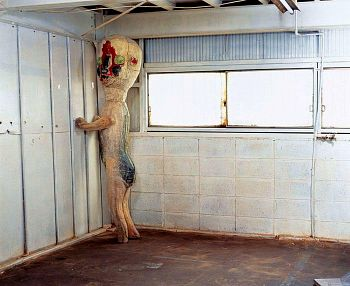
\includegraphics[scale=0.5]{illustration/SCP_173.jpg}
		
		\caption{\small \emph{Untitled 2004} créée par Izumi Kato. Cette photographie a été prise par Keisuke Yamamoto.}
		\label{img:scp_173}
	\end{wrapfigure}
	
	Durant plusieurs jours, SCP-173 s'est retrouvé copié puis collé (complétant ainsi, avec le caractère terrifiant son appellation de CP) sur le sous-forum /x/ puis sur la page d'accueil du site (le \textit{board} /b/), jusqu'à ce que d'autres utilisateurs se joignent au mouvement et produisent à leur tour d'autres CP inspirées par la forme et l'univers de cette CP originelle.
	C'est la suite de son cheminement qui fait passer cette histoire de simple CP à véritable canon : au fil des ans la communauté qui s'est construite autour de SCP-173 et de ce qu'on nomme désormais la \emph{Fondation SCP} s'est autonomisée, créant un wiki dédié (une première fois grâce au CMS \emph{EditThis} puis au CMS \emph{Wikidot}) puis continuant de croitre. Aujourd’hui la \emph{Fondation SCP} est présente dans 12 langues différentes et est forte de plusieurs milliers de productions originales dans chacune de celles-ci 
	
	Cette progression et ce rapport à une création de base peut nous amener à penser les CP comme une forme de fanfiction\footcite[voir p. 2]{goudet_agentivite_2021}.
	
	Ce rapprochement peut apparaître comme pertinent car, à l'instar d'un texte canonique source, les CP va être copié, annoté puis inévitablement modifié et ces modifications vont produire des textes à part entière. On note aussi la proximité en termes de moyen de production : l'écriture est collaborative en ce qu'elle produit une œuvre fragmentaire et asynchrone, chacun produisant à son rythme des éléments supplémentaires.
	
	De plus on trouve une dynamique similaire à celle que les fanfictions entretiennent avec le canon : l'idée de fanon\footcite{lata_du_2022} , où la production qui découle de l'œuvre originale (et donc canonique) va tirer son autorité de cette massivité\footcite{cook_canonicity_2013}. 
	Néanmoins cette analogie ne fonctionne que dans de rares cas. Les CP sont majoritairement des textes uniques, d'effrayantes bouteilles jetées à la mer par un utilisateur, qui n'a pas vocation à s'établir comme récit fondateur. 
	
	SCP-173 est donc un des rares exemple de cette trajectoire particulière : celle d'une CP prenant tellement d'ampleur qu'elle devient elle même la base d'un canon ou d'un \textit{fandom}. 

	
	Il n'existe que trois exemples de cette trajectoire : SCP-173 et la \emph{Fondation SCP}, les \emph{Backrooms} et \emph{Slenderman}. 
	Ces trois cas suivent une trajectoire similaire: une première publication sur un forum (respectivement \emph{4Chan} et \emph{SomethingAwful}), une vague importante de réaction sur ce même forum, puis une "exportation" vers une plateforme dédiée. Si la trajectoire globale est la même, chacune de ces CP a des caractéristiques formelles et "trajectorielle" propre (changement de forme et/ou de média).
	
	\subsection{Les CP historiques}
	
	Alors que toutes les CP ne suivent pas la même trajectoire qui restent largement exceptionnelles, certaines productions, dès les débuts de ce genre, ont laissé une empreinte indélébile sur le lectorat. Elles se sont hissées au rang de références, d'histoires marquantes qui ont contribué à définir le genre. 
	
	Ces CP, que nous qualifierons de CP \textbf{historique}, ont suivi un début de trajectoire similaire, mais ne se sont pas hissées au rang de canon. Malgré cela, elles ont connu un franc succès. Ce succès ne prend pas la forme d'histoires liées mais de reproductions sur d'autres formes. Au delà d'un simple copier-coller, ces histoires ont été narré sur d'autres plateformes,ou bien illustré sous différentes formes (animations, dessin...). 
	\textit{Ben Drowned}, que nous avons mentionné plus tôt, est un exemple de cette trajectoire : en plus de sa navigation sur différents forums, de nombreux utilisateurs, sur Youtube par exemple, utilise les images du jeux présentes dans la CP originale pour illustrer tout en narrant l'histoire associée\footnote{Voir par exemple \url{https://www.youtube.com/watch?v=2o7lcKHjdoQ\&pp=ygULYmVuIGRyb3duZWQ\%3D}}, ou ont cherché à expliquer, approfondir l'expérience\footnote{\url{https://www.youtube.com/watch?v=QJlqY1O4B00}}.
	On peut citer, à titre d'exemple, les CP \emph{le Syndrome de Lavanville} \footnote{\url{https://creepypasta.fandom.com/wiki/Lavender_Town_Syndrome}} qui évoque une rumeur sur la musique d'une version d'un jeu Pokémon, ou encore \emph{Squidward's Suicide} \footnote{\url{https://creepypasta.fandom.com/wiki/Squidward\%27s_Suicide}}, histoire d'un épisode disparu du dessin-animé \emph{Bob l'Éponge}.

	\subsection{Le reste des productions}
	
	Aujourd’hui néanmoins les différentes plateformes ne sont plus assujetties à une limite de maintien des données: ce faisant le mode de production et de diffusion des CP a évolué, et le copier-coller n'est plus un moyen de survie.
	
	Désormais, l’écrasante majorité des CP est produite sur des forums et sites dédiés (sans que cela soit néanmoins nécessaire, comme le montre l'exemple récent des \emph{Backrooms}, apparu la première fois sur \emph{4Chan}). Les deux pôles principaux de productions de CP sont aujourd'hui le \emph{subreddit} r/nosleep \footnote{\url{https://www.reddit.com/r/nosleep/}} et le fandom Creepypasta \footnote{\url{https://creepypasta.fandom.com/}}. 
	
	Ces deux plateformes voient quotidiennement de nouvelles histoires apparaître : ainsi si la diffusion et la viralité était un moyen de survie, les histoires produites sont désormais assujetties à des règles et des méthodes biens différentes. Ce faisant une nouvelle façon d'exister, une nouvelle trajectoire, s'est développée avec la sédimentation du "genre" au cours de ces dernières années. 
	Cette sédimentation à un double effet : avec l'affirmation du genre, est apparu la nécéssité de prendre en compte les auteurs de ces productions. Les production anonymes laissent leur place à des productions signées, voire en série, qui place les CP à nouveau dans une dynamique d'auctorialité plus traditionnelle, où l'auteur est replacé au centre \footnote{Il convient de noter néanmoins que ce régime d'auctorialité n'est pas le même dans le cadre des productions autour des super CP, qui forment, comme mentionné plus tôt une sorte de fanon, et donc diffuse l'auctorialité par la même.}.
	
	Il convient néanmoins de noter dès maintenant une différence cruciale dans le fonctionnement de ces deux plateformes : en plus d'accueillir du contenu produit régulièrement le fandom Creepypasta joue aussi un rôle d'"archive" des CP historiques. 
	
	Cette sédimentation, liée à la production massive de CP \footnote{Le Fandom compte près de 14 000 pages}, entraîne aussi une attente différente vis à vis de la qualité des productions : d'un genre spontané, la CP s'est construite au fur et à mesure comme un genre travaillé. \footcite{garcia_roca_creepypasta_2021}
	
	Les plateformes accueillant ces productions ont donc développé des standards de création devant être respectés sous peine de ne pas pouvoir publier. 
	
	A défaut de rentrer dans la description des règles de ces plateformes, l'existence même de celles-ci est intéressante : il existe désormais une attente liée à la qualité et littérarité des CP. Cette littérarité, comme nous l'avons laissé sous-entendre, n'est pas évidente : des productions anonymes sur des canaux de diffusion nouveaux et souffrant encore d'un manque de légitimité \footcite{saemmer_litterature_2011} sont autant d'indice quant à un décalage entre les productions littéraires patrimoniales et les productions numériques.
	
	
	

		\part{Récupération et traitement des données}
		
		\chapter{Récupération : moissonnage des plateformes}
	
	La récupération des données a nécessité une méthode différente pour chacune des plateformes.  En effet, le moissonnage des données présentes sur le web est dépendant à la fois de la forme de la plateforme et des données qui y sont présentes tout comme de la potentielle politique d'utilisation et de récupération de celle-ci. 
	
	\section{Le Fandom Creepypasta}
	Pour ce qui est du fandom CP, la récupération des données a été relativement facile : le site n'est pas structuré sous la forme d'un arbre, comme on pourrait s'y attendre. Au contraire, une grande partie du site, dont les histoires à récupérer font parties, n'est pas hiérarchisée. Ce faisant, il n'est pas possible d'utiliser l'organisation du site pour repérer et récupérer les différentes publications.
	Cette structure ne permet pas une méthode "brutale" qui consisterait à récupérer l'ensemble du site puis filtrer les pages qui nous intéressent en fonction du lien.
	
	A défaut de hiérarchisation, le site utilise une structure par hyperlien, où les pages sont organisées autour d'autres pages centrales, qui permettent par exemple de référencer certaines catégories. Ainsi pour accéder à une partie du site il faut : la chercher explicitement ,ou dans la plupart des cas, y accéder en appuyant sur un lien présent sur un page. 
	Ainsi, afin de récupérer les publications, il est nécessaire de trouver une page qui renverrait vers toutes les autres publications. Par chance, une telle page existe sur le site : cette page a néanmoins la particularité de ne pas être accessible depuis la page d'accueil.
	A partir de cette page la méthode de récupération est la suivante: dans un premier temps on récupère l'ensemble des liens des pages, puis on récupère les données au sein des pages qui nous intéresse. 
	Pour ce faire, les bibliothèques Python \emph{Selenium} et \emph{BeautifulSoup} ont été mobilisé: ces deux bibliothèques permettent respectivement de naviguer au sein des pages en simulant le comportement d'un utilisateur, et de récupérer les informations dans le code des pages. 
	Afin de naviguer à travers la page de référence, il suffit de "cliquer" sur le bouton page suivante (action réalisée à l'aide de \emph{Selenium}). Une fois toutes les pages collectées, il faut récupérer la partie qui nous intéresse : le corps du texte. 
	Nous avons utilisé la fonctionnalité d'édition du site à notre avantage: cette fonctionnalité permet d'afficher le texte brut, sans mise en page. De plus, cette représentation place le texte dans une zone mieux délimitée dans le code source, tout en donnant accès à des informations moins accessibles : les catégories par exemple, mais aussi l'auteur s'il est mentionné. 
	\begin{figure} [htbp]
		\centering
		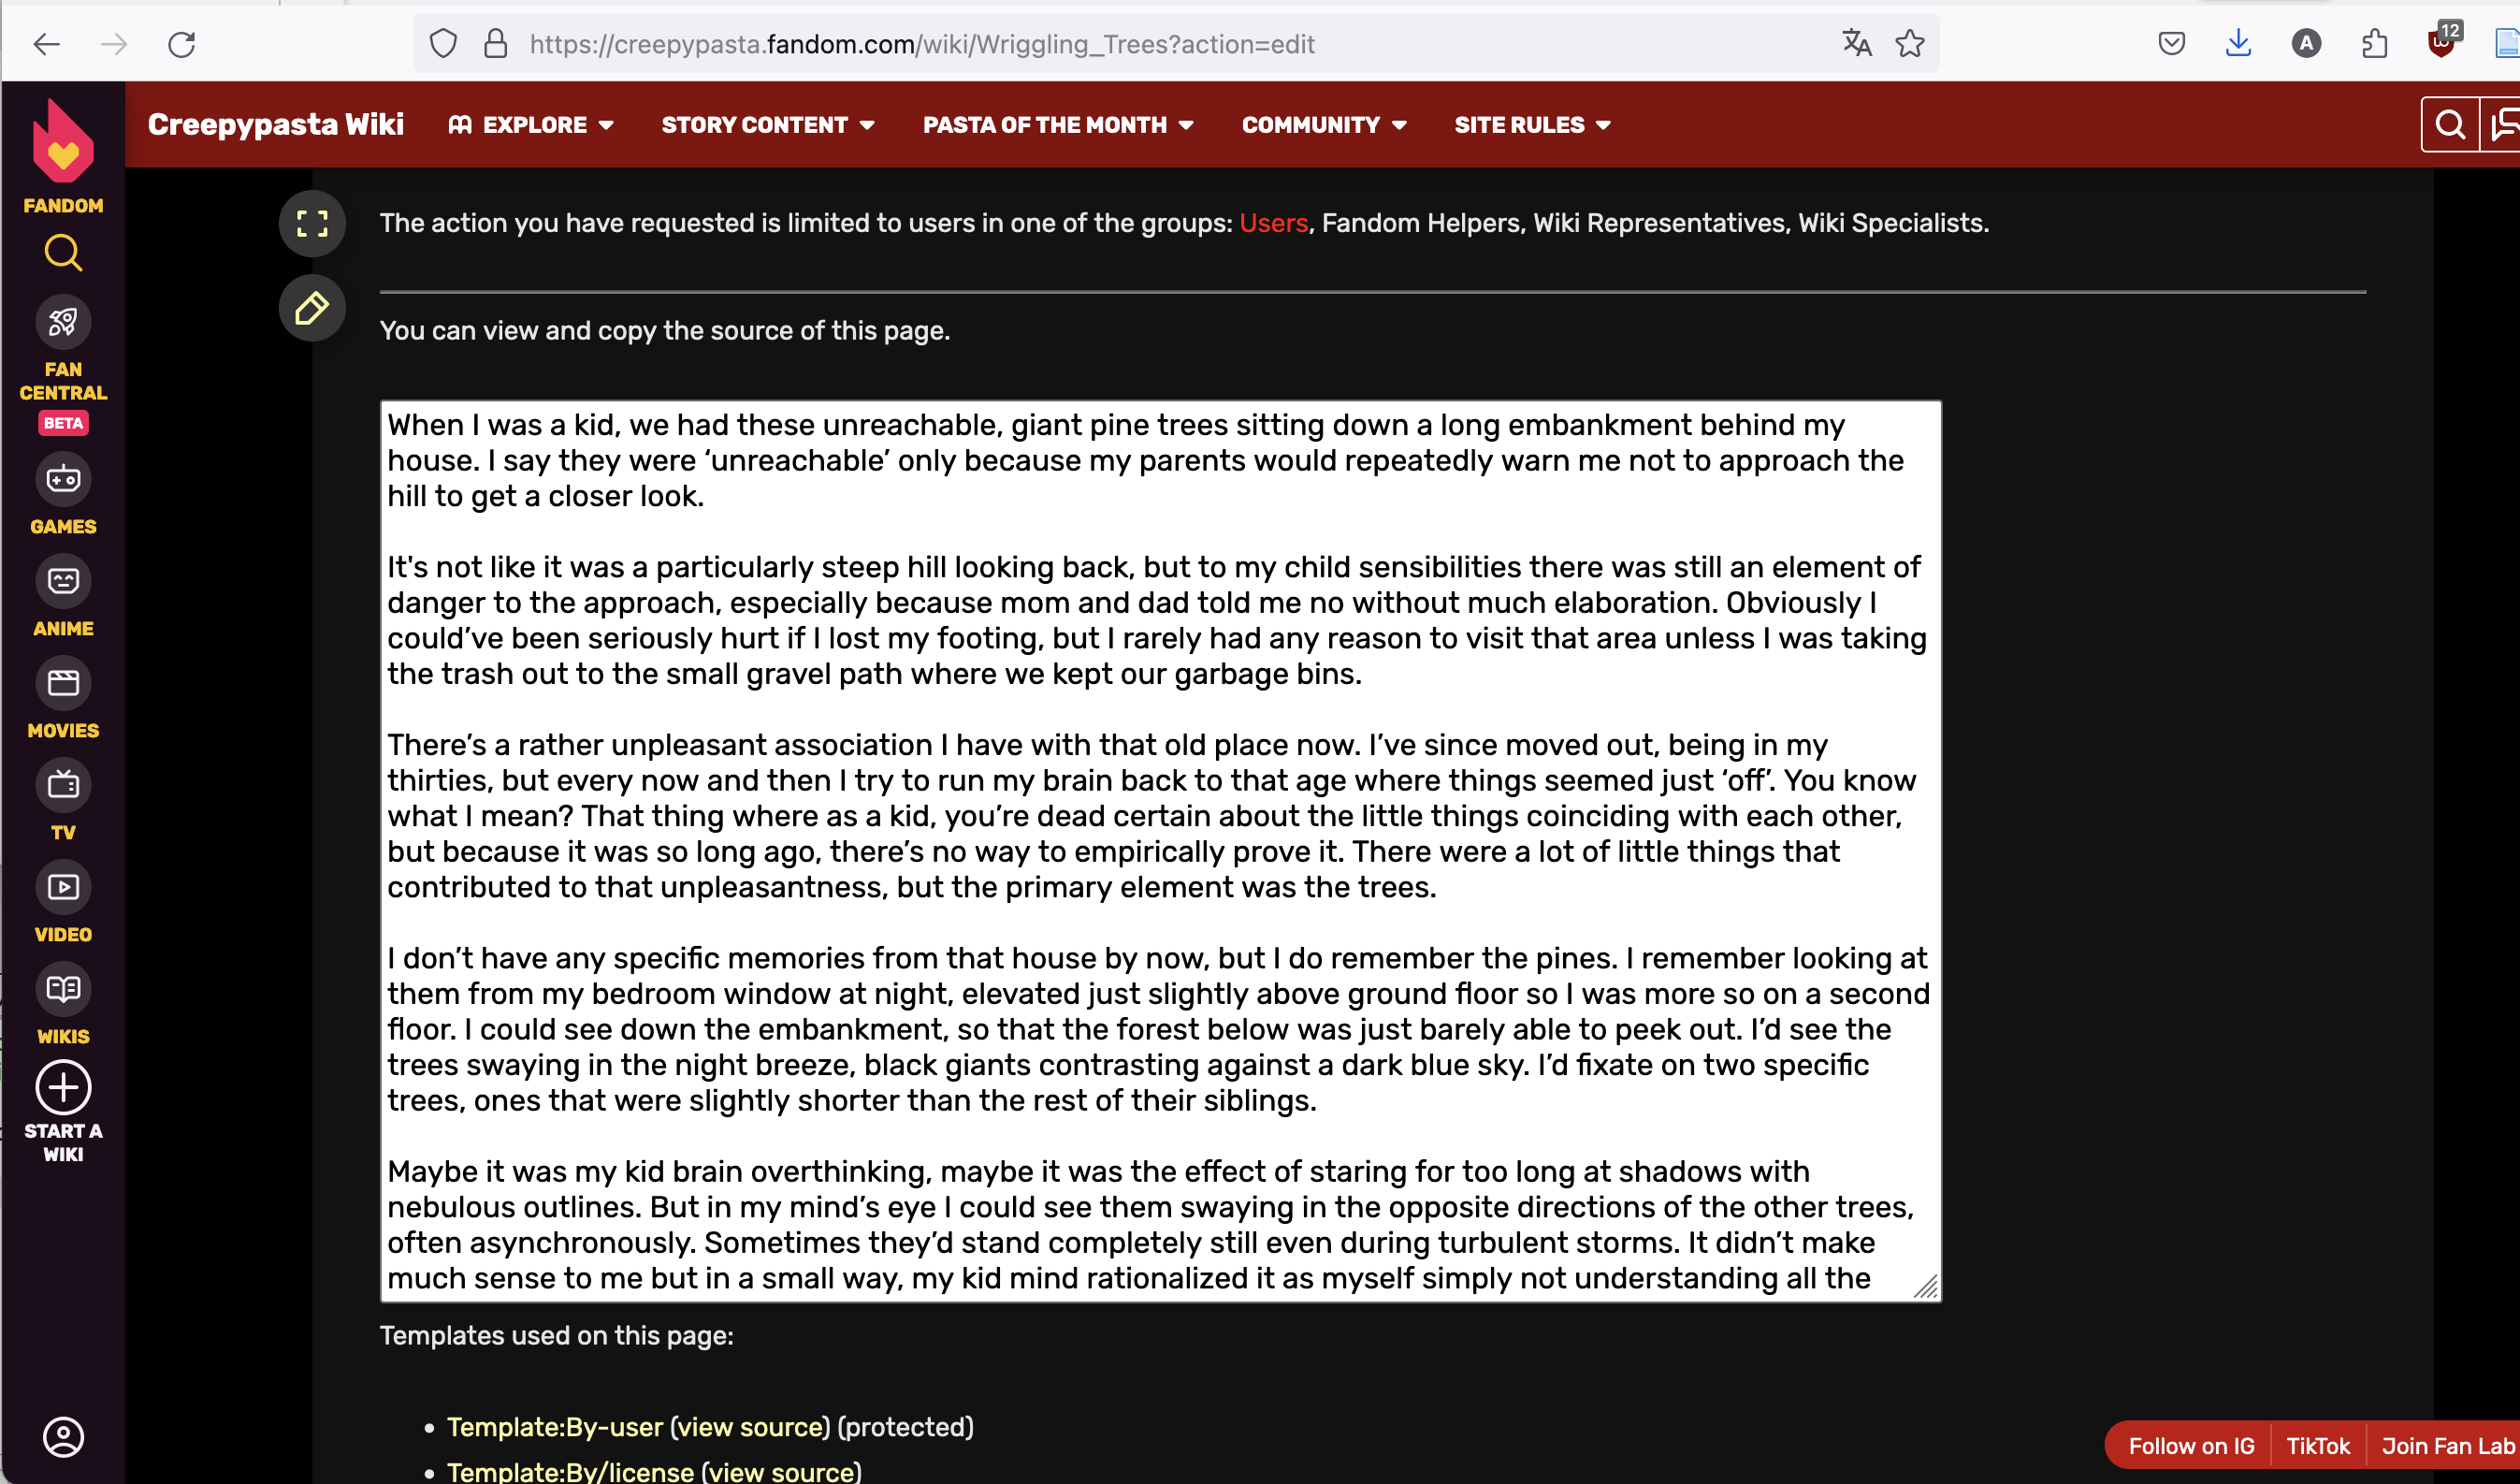
\includegraphics[scale=0.2]{illustration/site_edit.png}
		\caption{Page d'édition d'une des CP du site : la zone en blanche correspond au corps du texte}
	\end{figure}
	
	Une fois la récupération de donnée effectuée, les textes bruts et les métadonnées (date, catégories, auteur) sont structuré puis stocké dans un fichier à part, au format .csv .
	
	\section{Le subreddit /r/nosleep}
	Pour ce qui est du subreddit, la marche à suivre pour récupérer les textes et les données associées est sensiblement différente. D'une part, \emph{reddit} dans son entiereté est un site à l'affichage dynamique : autrement dit, les données apparaissent au fur et à mesure que l'utilisateur progresse sur la page, et ne sont pas à une place défini. A cela s'ajoute une limite d'affichage arbitraire définie par le site (en l'occurrence, il n'est pas possible d'afficher plus de 1000 publications à la fois). 
	Outre la difficulté de récupération des données, ces limites ne permettent pas de saisir la taille réelle du subreddit\footnote{Les évolutions récentes de la politique de gestion des données de la plateforme a rendu presque impossible la collecte automatique de données et de statistiques. Ainsi des sites spécialisés comme \url{https://subredditstats.com} ne sont plus à jour} : la seule donnée disponible est le nombre de membres du subreddit. Si cette donné est importante, elle n'est qu'une indication indirecte sur le nombre de publications (chaque membre ne publiant pas nécesseraiement). 
	Ce moissonage nous a permis de récupérer l'ensemble des production du site, soit près de 13000 publications (13128 pour être exact).
		
	Pour le premier moissonnage,nous avons décidé de récolter les publications au nombre de vote le plus élevé, indépendemment de la date. En effet, contrairement à la plateforme \textit{Fandom}, reddit dispose d'un indicateur quantitatif quant à la réception d'une publication : cette information nous permettra par la suite d'explorer les inférences entre réussite et forme.
	De cette manière , nous avons récupéré un millier de pages. 
	
	S'il est possible de considérer que les presque 14000 produtions récupérées sont suffisantes, le déséquilibre important entre les corpus risque de biaiser les résultats. De plus, le fait d'avoir sélectionné les productions les mieux notées de la plateforme reddit est intéressant, mais risque là encore de mener à un biais important quant à la caractérisation des corpus : on peut supposer que les caractéristiques textuelles des meilleures production ne reflètent pas nécessairement les caractéristiques de toute la plateforme.
	
	Néanmoins, une recherche plus approfondie nous a permis de découvrir la base de données Pushshift\footcite{baumgartner_pushshift_2020}, base de données recensant les productions de l'ensemble des subreddit de 2005 à 2019. Ainsi de 1000 publications, nous avons été capable de récupérer pas loin de 190000 publications\footnote{le total de publication s'élève dans les fait à 385668 productions. Néanmoins plus la moitié a été supprimé ou retiré de la plateforme.}, nous permettant par la même de déterminer le nombre de production totale sur cette période. 
	Or un tel nombre de productions n'est pas sans problème : de pas assez nous sommes arrivés à trop. Cette masse de données considérables rend les computations beaucoup plus gourmandes, trop pour l'ordinateur utilisé du moins, et représente un obstacle conséquent. Ainsi pour palier à cette limite, nous avons sélectionné des échantillons afin d'équilibrer le corpus. Pour construire cet échantillon nous avons procédé en deux temps, en sélectionnant une première partie de l'échantillon en fonction de la date, puis en sélectionnant l'échantillon en fonction de la note. En sélectionnant respectivement 7500 publications réparties équitablement sur l'ensemble du corpus, nous avons réussi à obtenir un corpus mieux équilibré et suivant la même répartition dans le temps et sur les notes. 
	
	Enfin nous avons agrégés les données échantillonnées du \textit{subreddit} avec celle obtenue sur le Fandom, afin de produire notre base de données de départ.
	
	
	
	\chapter{Traitement des données}
	Comme nous l'avons laissé sous-entendre, notre traitement sera un traitement exclusivement textuel. Et une des premières notions que nous avons cherchées à aborder est la littérarité.
	
		La question de la littérarité ("c'est-à-dire ce qui fait d'une œuvre donnée une œuvre littéraire" \footcite{aron_litterature_1984}) est, d'un point de vue quantitatif (et donc du point de vue de la forme et non du fond), définissable sous différentes formes: le but est de mettre en avant une complexité textuelle caractéristique des œuvres littéraires, des caractéristiques qui différencieraient les textes de simple publication sur un forum.
		
		De précédentes recherches ont montré à la fois la capacité à modéliser la littérarité\footcite{koolen_literary_2020} et quels éléments du texte pouvaient servir à l'évaluation de la littérarité\footcite{van_cranenburgh_identifying_2015}. Dans le cadre de notre étude, nous commencerons par voir si des indices plus simples et plus facilement obtenables suffisent à caractériser le caractère littéraire des productions, sans exclure la possibilité future d'appliquer les dites méthodes\footnote{pour un aperçu des avancées dans le domaine des études du canon computationnelles voir \footcite{barre_operationalizing_2023}}.
		

		Dans cette optique nous mobiliserons et de comparerons des métriques comme la longueur des texte, la taille des phrases, la complexité du vocabulaire ou des indices lisibilité (\textit{readability}). 
		En plus des témoins syntaxiques, nous mobiliserons également des données sur le fond des textes : ainsi s'ajouteront à cela une analyse des thèmes et des sentiments présents dans les textes.
		Il peut être intéressant de déterminer si ces différents indices sont présents/absents de la même manière sur les différentes plateformes, lorsque cela est pertinent : cette analyse permettra de dresser la présence ou l'absence de similarité dans la forme au sein des différentes plateformes, et donc de déterminer une forme d'autorité propre à chaque plateforme.\footcite{mayer_autorite_2017}. 
	
		Enfin, une dernière comparaison apparaît comme féconde : à défaut d'avoir une indication quantitative du succès des publications sur le fandom, une donnée qualitative (le caractère "historique") va nous permettre d'isoler un sous-corpus.  
		L'existence de ce corpus nous permettra de tester les hypothèses d'évolutions et de caractérisation plus en profondeur: est-ce que ces CP ont émergé au sein d'une tendance, ou est-ce qu'au contraire, ce sont elles qui ont permis l'émergence d'une tendance ? 
		
		Afin de comparer de prendre la mesure des valeurs, nous avons sélectionné deux corpus de référence, un littéraire \footnote{\url{https://github.com/computationalstylistics/100_english_novels/tree/master/corpus}} et un issu de l'agrégation de données issues de différents sites internet \footnote{\url{https://www.english-corpora.org/iweb/}}. Le genre appartenant théoriquement à ces deux domaines, la comparaison va nous permettre de situer les CP vis à vis de ceux-ci. Ce sera l'occasion aussi d'éviter les conclusions hâtives: la longueur des phrases ou la lisibilité sont-elle propres au CP, ou, au contraire, sont-elles simplement conformes à ce qui se trouve sur internet dans son ensemble.
		
	\part{Premiers résultats}
	
	\chapter{Caractérisation des Creepypastas}
	
	
	\section{Longueurs et longueurs des phrases}
	Un des premiers éléments caractéristique des creepypastas, d'après la définition d'Ondrak citée précédemment, est la petitesse des productions. 
	
	\begin{figure}[htbp]
		\centering
		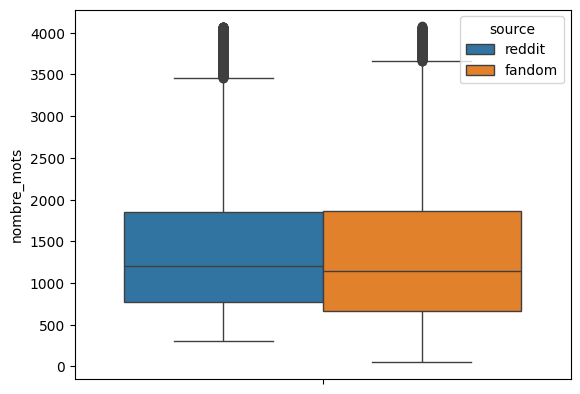
\includegraphics{illustration/boxplot_nombre_mots.png}
		\caption{Boîte à moustache des valeurs du nombre de mots par productions}
	\end{figure}
	
	Avec une médiane à presque 1179 mots et une moyenne à 1390 mots, les productions des différentes plateformes sont courtes : à titre de comparaison, un roman, en moyenne, contient entre 50 000 et 100 000 mots.
	Concernant les deux plateformes, on ne note pas de différence significative entre les deux : elles semblent être relativement homogènes. 
	
	Autre élément qu'il est intéressant d'analyser, la longueur moyenne des phrases. Cet élément est souvent associé à la littérarité : plus la phrase est longue, plus la phrase peut être complexe. 
	
		\begin{figure}[htbp]
		\centering
		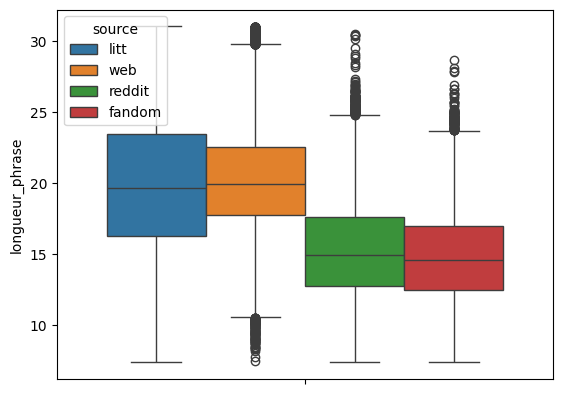
\includegraphics{illustration/boxplot_phrases.png}
		\caption{Comparaison de la dispersion des longueurs moyenne des phrases en fonction des corpus}
	\end{figure}
	
	Le premier élément qui nous apparaît est la différence significative entre les corpus web et littéraire d'un côté, et des CP de l'autre. Si nous retrouvons à nouveau une différence négligeable entre les plateformes, les phrases des CP sont en moyenne bien plus courtes. 
	Cette conclusion semble aller dans le sens d'une littérature qui incorpore avant tout les codes de la viralité au détriment de la littérarité : les phrases sont en moyennes plus courtes et restent, du point de la dispersion, plus basses que les phrases littéraires. Ce constat est d'autant plus frappant lorsqu'on ajout les données issues du web : si on pouvait faire l'hypothèse d'une complexité plus faible pour le web, celle-ci se trouve invalidée dans un premier temps et accentue l'importance des phrases courtes relativement pour les CP.


	\section{Topic Modelling}
	\label{section_topic}


    %% Ajouter expérimentation avec BERTopic pour permettre une quantification des résultats + comparaison de la pertinence des résultats
	
	Afin de caractériser au mieux les productions, un bon moyen est d'identifier puis d'analyser les thèmes les plus fréquents. Comme nous l'avons mentionné précédemment, les CP se démarquent d'une part par leur forme, mais aussi par les thèmes précis (numérique, vie de tous les jours...). Ainsi cette analyse va nous permettre de vérifier cette hypothèse à l'échelle du corpus et non pas de quelques exemples marquants. 

	Pour ce faire, nous avons employé une méthode de \emph{Topic Modeling} basée sur une vectorisation TF-IDF des textes du corpus puis d'une détection de communauté en utilisant de l'algorithme de Louvain afin d'isoler les communautés sémantiques comptant le plus de documents. 

%% Ajouter une meilleure description de la méthode (ajouter un schéma ?), avec explication du choix du seuil
	
	Par cette méthode,  nous avons isolé les douze thèmes suivants (cf. Figure \ref{fig:topic_corpus}) : 
	\begin{itemize}
		\item le sommeil
		\item la douleur physique
		\item les animaux de compagnie
		\item la voiture, transport automobile
		\item l'enfance
		\item la famille
		\item la jeunesse (école, amitié...)
		\item les jeux-vidéos, la technologie
		\item la forêt
		\item miroir et reflet
		\item les araignées
		\item expériences traumatiques\\

		\end{itemize}

	Parmi ces thèmes, on remarque ceux précédemment évoqués : la technologie et les jeux-vidéos et l'enfance à travers la famille. D'autres thèmes néanmoins sont peut-être moins attendus, plus surprenants pour des productions à vocation horrifique : si les araignées, la souffrance physique, et le traumatisme sont attendus, l'importance de la famille par deux thèmes distincts ou bien les animaux de compagnie est remarquable. 
	Ces thèmes apparaissent comme ayant un point commun : un rapport étroit avec l'expérience personnelle. La famille, la souffrance, et le foyer sont autant d'éléments relevant de l'intime. 
	De la même façon, le miroir ou la forêt mobilisent un symbolisme assez proche : le miroir d'abord est un lieu de révélation, de prise de conscience, voire d'affrontement \footcite[voir p.639, article "Miroir"]{chevalier_dictionnaire_1990}, là où la forêt est un lieu symbole de l'inconscient et de la crainte de celui-ci, comme plus prosaïquement, un lieu de mystère \footcite[voir p.455, article "Forêt"]{chevalier_dictionnaire_1990}


	\begin{figure}[htbp]
	\centering
	\begin{subfigure}{0.45\textwidth}
		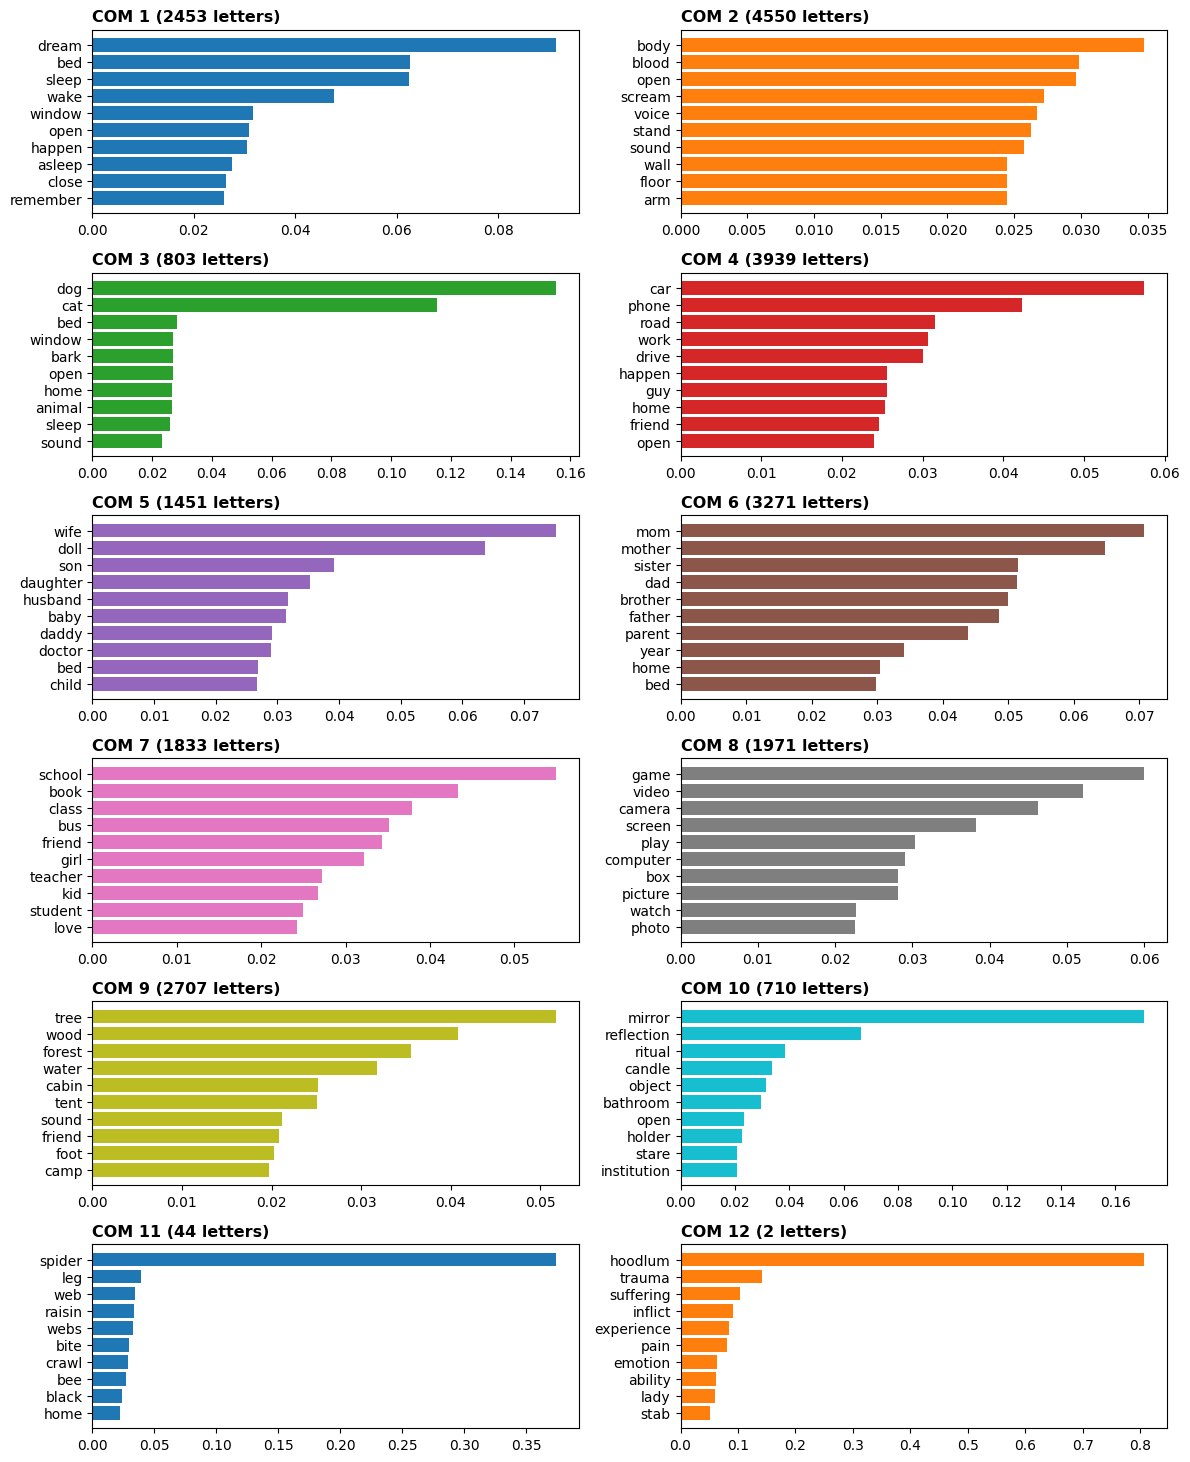
\includegraphics[width=\textwidth]{illustration/tf_idf_topic_corpus_variables.png}
		\caption{Topic les plus fréquents sur l'ensemble du corpus}
		\label{fig:topic_corpus}
	\end{subfigure}
	\hfill
	\begin{subfigure}{0.45\textwidth}
		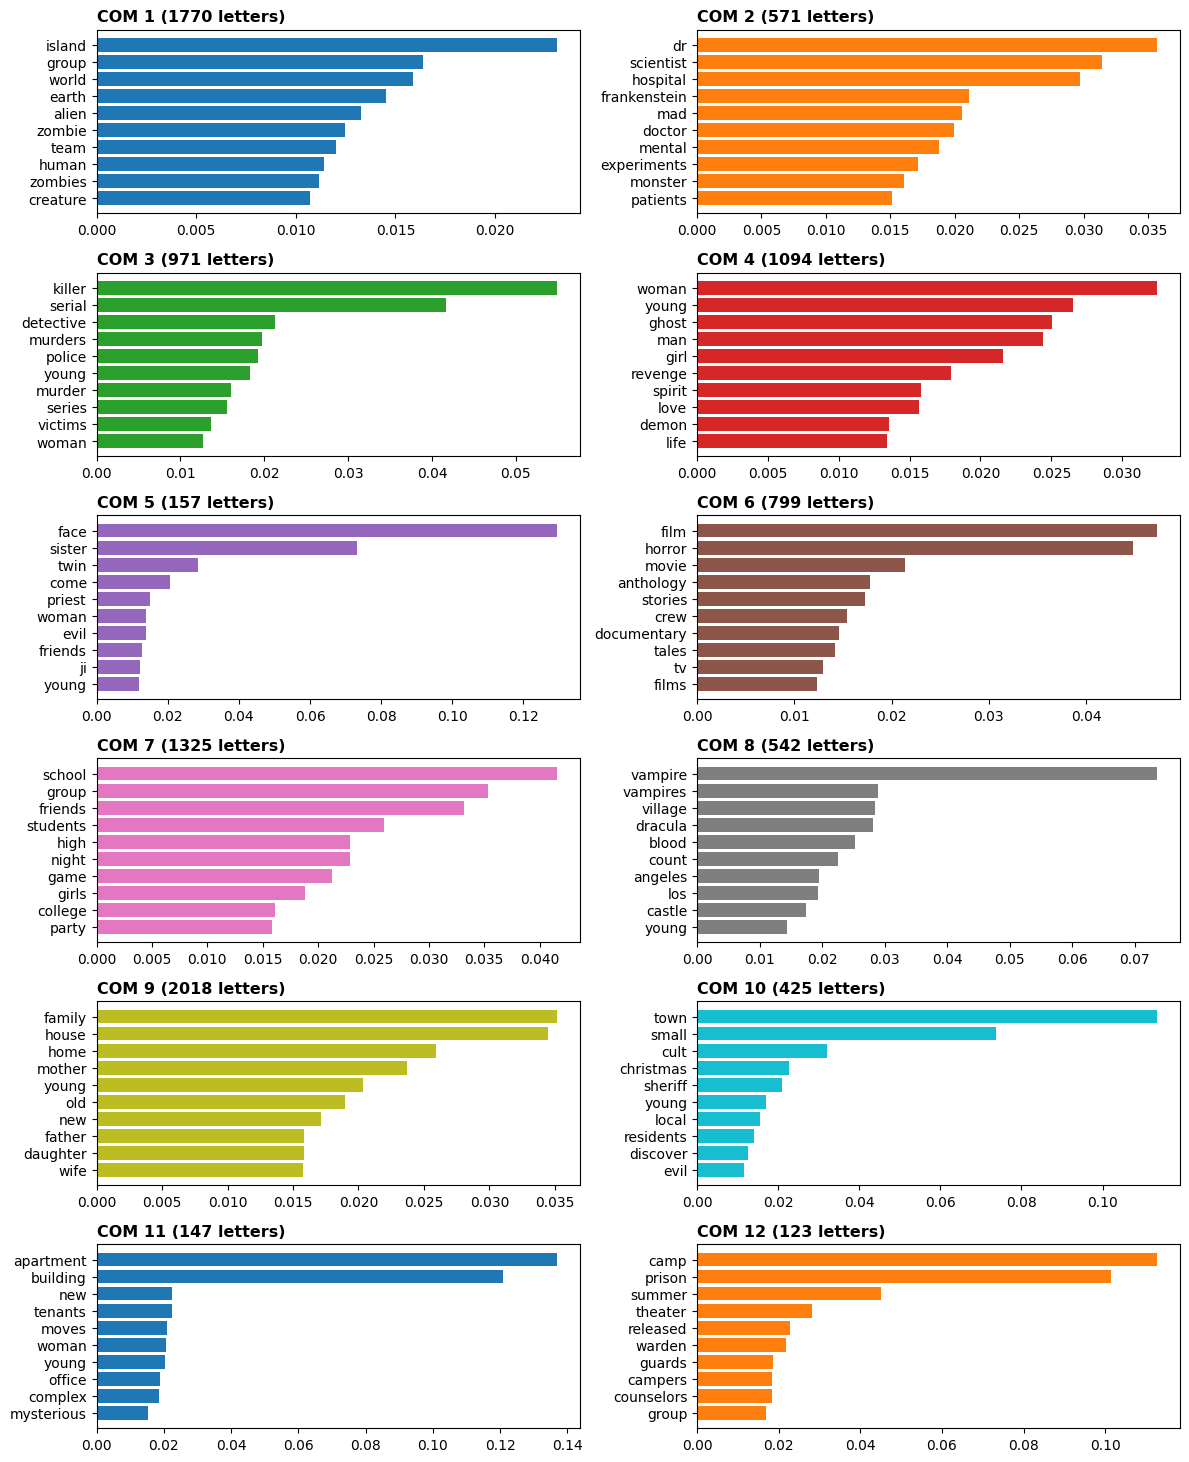
\includegraphics[width=\textwidth]{illustration/tf_idf_topic_tmdb.png}
		\caption{Topic les plus fréquents des films d'horreur de \emph{TheMovieDataBase}}
		\label{fig:topic_tmdb}
	\end{subfigure}
	\caption{Visualisation des topics les plus fréquents de deux corpus}
	\label{fig:topics_corpus}
	\end{figure}
	
	Afin de souligner à quel point ces thèmes sont caractéristiques de ce genre de littérature d'horreur, nous avons cherché à identifier les thèmes les plus récurrents des productions cinématographiques d'horreur.
    %%Ajouter le fait que c'est un des médium privilégier pour le genre, avec statistiques à l'appui 
	Pour ce faire, nous avons suivi la même méthode d'extraction des thèmes cette fois-ci sur un ensemble de descriptions de films d'horreur extrait de la base de données \textit{The Movie Data Base}\footnote{\url{https://www.themoviedb.org/}} (cf. Figure \ref{fig:topic_tmdb})	
	
	La différence entre les thèmes est flagrante : si les CP évoquent en filigrane l'expérience personnelle, le foyer, l'intimité , les films d'horreur sont plus facilement tournés vers le spectaculaire et le surnaturel (zombie, expérience scientifique, religion, vampire). 
	Ainsi l'hypothèse d'un genre caractérisé par un lien étroit avec l'intimité et l'expérience semble se confirmer : le frisson de l'horreur ne passe que rarement par des effusions de sang, mais bien par quelque chose de plus subtil.
	De plus, les thèmes des CP sont doubles, étant à la fois élément de cadre et potentiellement éléments déclencheurs de la peur. Cette dualité n'est pas présente, ou dans une dimension moindre dans un film d'horreur par exemple . Un zombie, élément déclencheur de la peur par excellence, n'est pas nécessairement un élément cadrant du récit, du moins pas au même titre que la famille par exemple, qui peut aussi bien être un thème cadre, et ce qui, une fois pervertie ou distordues, apporte l'élément horrifique. Dès lors, on peut supposer que la subtilité des thèmes et de l'horreur est double : la peur n'est pas issue d'élément spectaculaire et infuse donc le récit.
	
	Notons aussi que cette caractérisation n'est pas dépendante de la plateforme d'origine : à quelques différences près, les thèmes présents sur les deux plateformes sont les mêmes (cf. Figure \ref{fig:topic_CP} et Figure \ref{fig:topic_reddit}). 
	
		
		
		\begin{figure}[htbp]
			\centering
			\begin{subfigure}[b]{0.45\textwidth}
				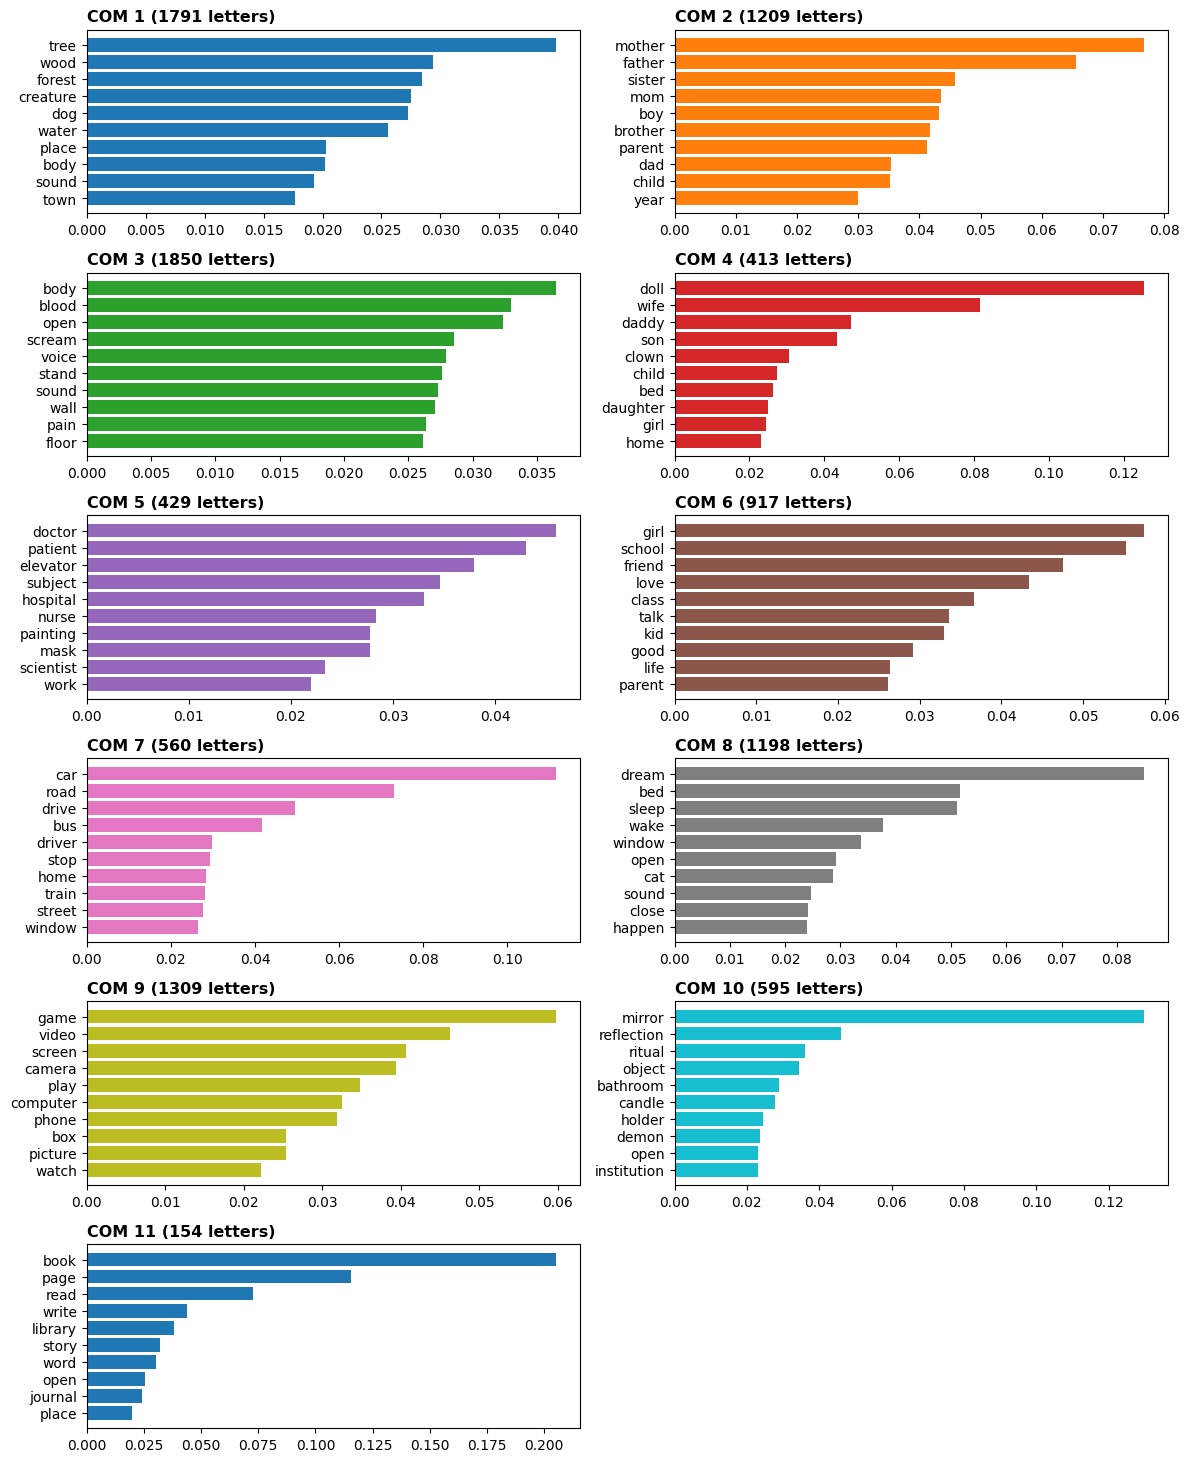
\includegraphics[width=\textwidth]{illustration/tf-idf_topic_fandom.png}
				\caption{Topic les plus fréquents du \emph{Fandom Creepypasta}}
				\label{fig:topic_CP}
			\end{subfigure}
			\hfill
			\begin{subfigure}[b]{0.45\textwidth}
				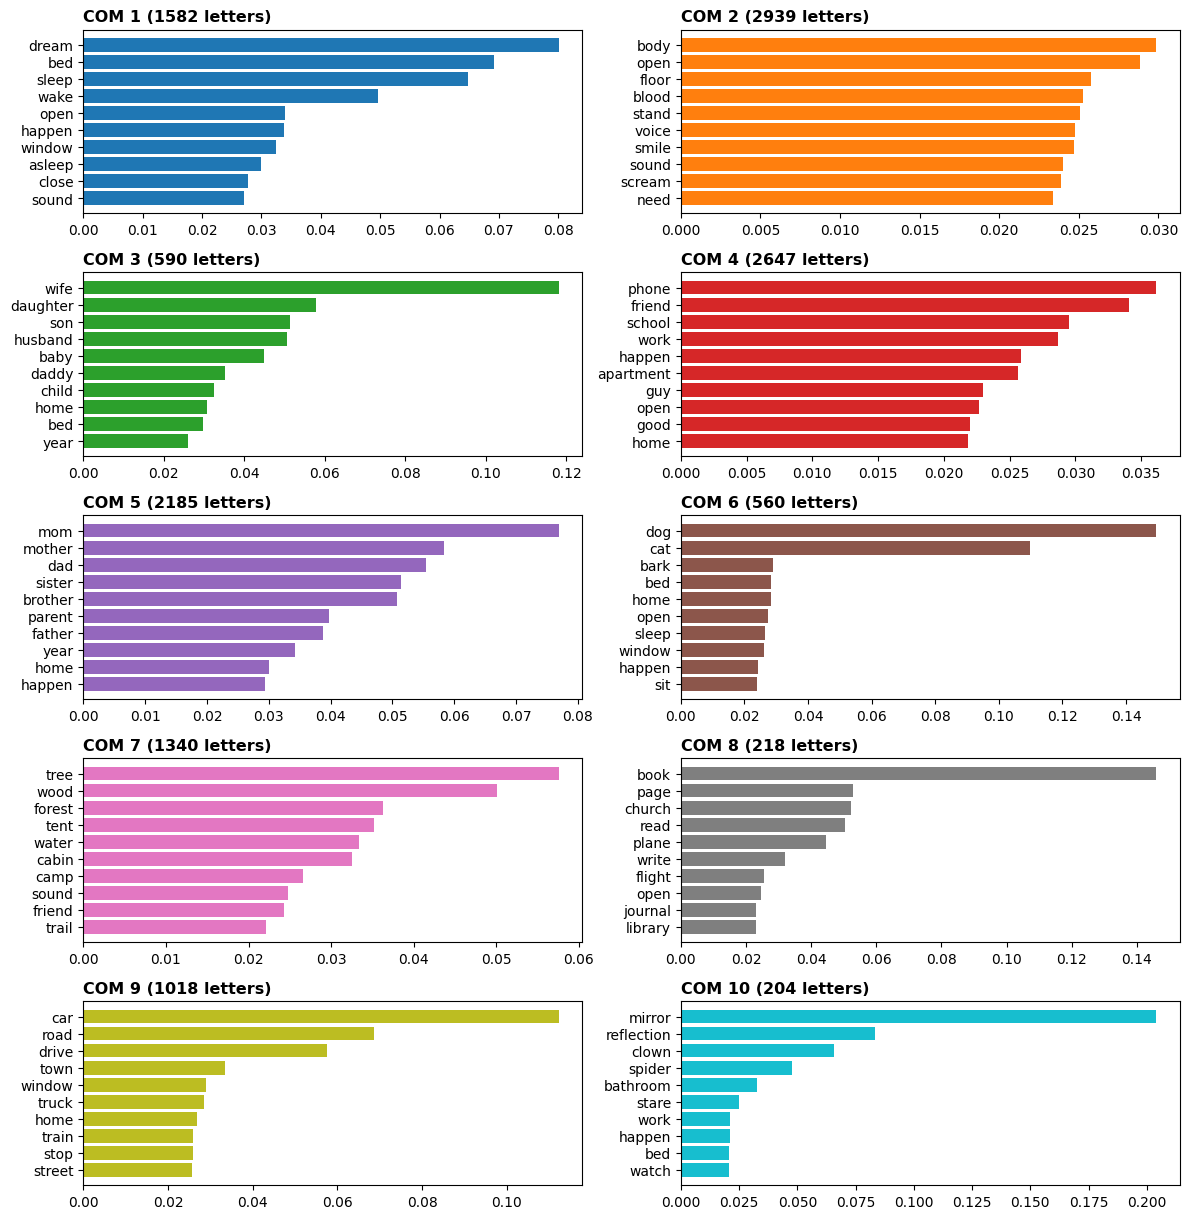
\includegraphics[width=\textwidth]{illustration/tf-idf_topic_reddit.png}
				\caption{Topic les plus fréquents du subreddit /nosleep}
				\label{fig:topic_reddit}
			\end{subfigure}
			\caption{Visualisation des topics les plus fréquents en fonction de la plateforme d'origine}
			\label{fig:topics_plateforme}
		\end{figure}
		

	% richesse lexicale et lisibilité
	\section{Mesurer la complexité d'un texte : Richesse Lexicale et indice de lisibilité}
	
	Une manière de mesurer le caractère littéraire d'une œuvre réside dans la mesure de sa complexité. Mesurer la complexité d'un texte peut se faire de plusieurs manières. Dans une perspective quantitative, nous avons sélectionné deux types d'indicateurs : les indices de lisibilités et les indices de richesses lexicales. 
	Pour rendre l'étude de ces indices plus pertinentes les résultats seront comparés à nouveau au corpus Web et de littérature anglaise.


	\subsection{Les indices de lisibilités} 
	Les indices de lisibilité sont des indices calculés afin de mesurer la difficulté de lire un texte. Le plus souvent, la valeur de ces indices est associée à un niveau scolaire : en effet, ces indices sont souvent un moyen de rendre compte de la difficulté d'un texte dans le cadre pédagogique.
	En ce qui nous concerne, notre but est d'une part de caractériser la lisibilité des CP, tout en rendant compte de la difficulté relative de lecture. Comme nous l'avons mentionné précédemment, nous faisons l'hypothèse d'une lisibilité relativement élevée, en lien avec une prétention grandissante à la littérarité. Nous nous attendons donc à voir apparaître une lisibilité plus élevée (c'est à dire une plus grande difficulté de lecture) vis à vis du corpus Web, mais plus faible vis à vis du corpus littéraire.
	
	\begin{figure}
\centering
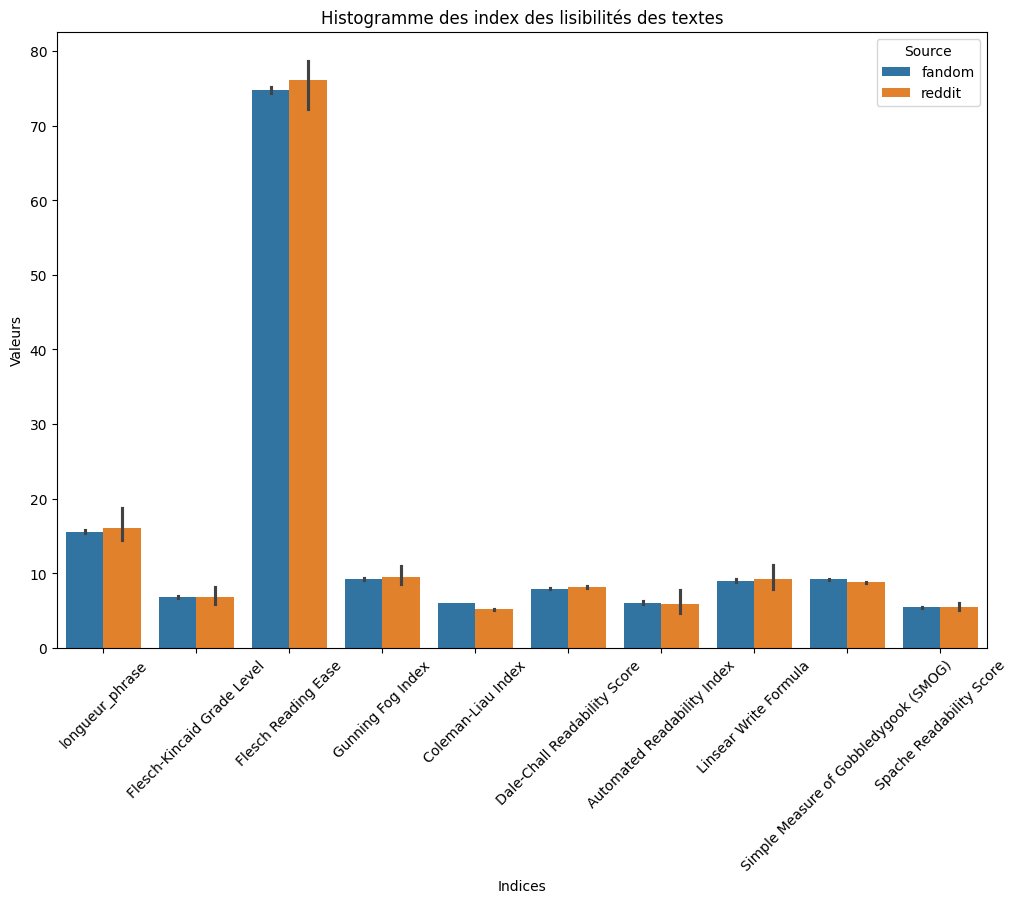
\includegraphics[scale=0.45]{illustration/comparaison_lisibilite_source.png}
\caption{Moyenne des indices de lisibilités sur le corpus}
\label{fig:mean_readbility}
	\end{figure}
	
	Avant de comparer les résultats, il convient d'analyser les valeurs de ces indices. Pour celles-ci, les valeurs correspondent au niveau scolaire théorique adapté pour la lecture dudit texte. Plus l'indice est haut, plus le texte est exigeant. Pour les équivalence entre les valeurs et le niveau scolaire voir les table \ref{tab:readability_indices_part1} et table \ref{tab:readability_indices_part2}.
	

	Pour ce qui est des valeurs, on note pour tous les indices des valeurs basses, du moins plus basses que ce à quoi on pourrait s'attendre d'un genre littéraire (cf. Figure \ref{fig:mean_readbility}): Les indices oscillent entre un niveau scolaire primaire ou secondaire, soit des textes accessibles à des jeunes collégiens. 
	
	
	Ces faibles valeurs sont d'autant plus importantes qu'elle le sont aussi de façon relatives (cf. Figure \ref{fig:comparaison_readability}): en comparant à nos deux corpus de référence, on observe des valeurs significativement plus basses aussi bien vis à vis de la littérature que du web. 
	Peut être le plus intéressant reste la différence observable entre notre corpus et le reste du web : s'il est possible d'expliquer partiellement les valeurs élevées de lisibilité du web par la forme de la source (c'est à dire un ensemble hétérogène de données textuelles, ce qui explique la dispersion des données), il n'en reste pas moins que notre corpus apparaît comme plus accessible. Ce qui peut  apparaître comme pertinent : une littérature caractérisée par la viralité se doit d'être lisible facilement afin d'atteindre le plus de monde possible, ce qui est appuyé par la conclusion vis à vis de la longueur moyenne de phrases.
	
	
	
	\begin{figure}
		\centering
		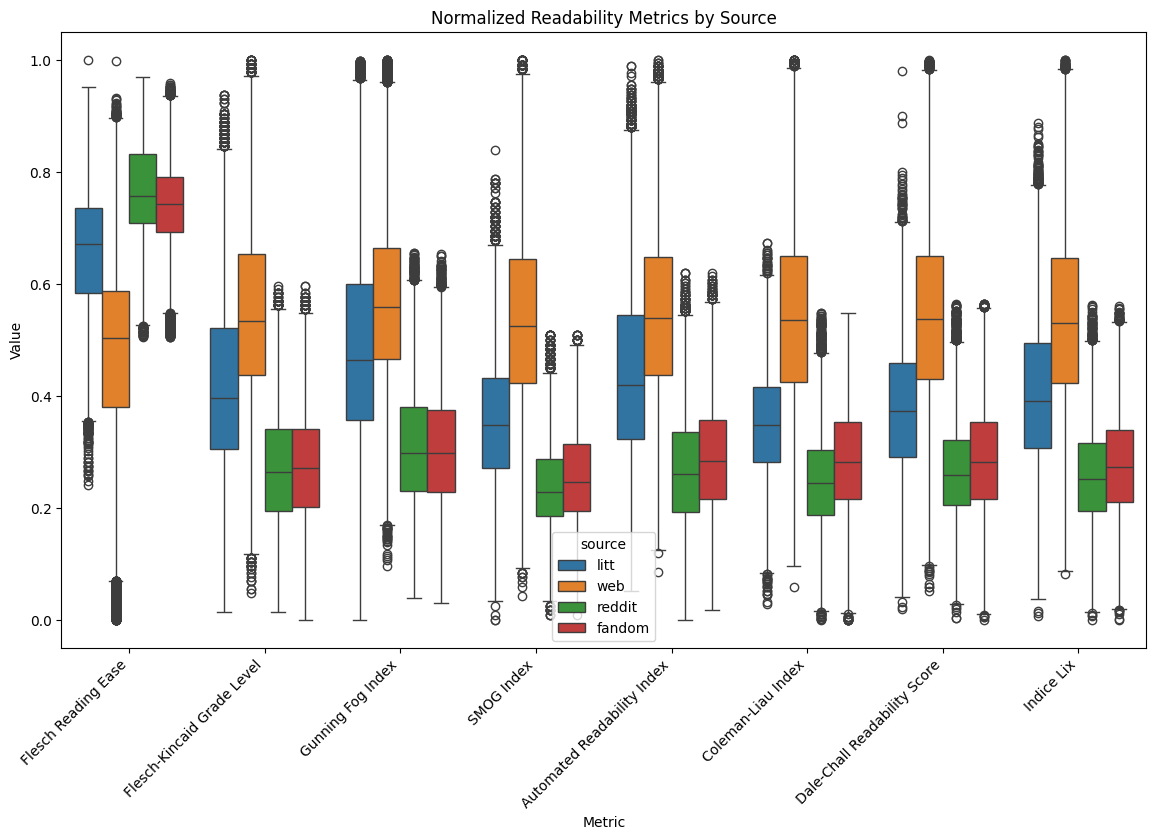
\includegraphics[scale=0.45]{illustration/boxplot_readability_V2.png}
		\caption{Comparaison des indices de lisibilités normalisés entres les différentes sources}
		\label{fig:comparaison_readability}
	\end{figure}
	
\pagebreak
	
	
	
	%Comparaison des richesse lexicales 
	\subsection{Les indices de richesse lexicales}

Allant de pair avec la difficulté de lecture, les indices des mesures lexicales sont, comme leur nom l'indique, des mesures de la richesse du vocabulaire. Bien que chaque indice fonctionne différemment (cf. Partie \ref{annexe_richesse_lex}), le principe reste similaire : on compare le nombre total de mots ou de tokens à un élément spécifique. Nous avons sélectionné initialement quatre indices (cf. \ref{annexe_richesse_lex}).

Intuitivement, nous avons cherché à utiliser cette mesure pour mettre en évidence, de la même manière que les indices de lisibilité, une certaine littérarité. En effet, un texte littéraire, et donc plus complexe, est supposé utiliser des mots plus rares et en plus grand nombre, en plus d'avoir une structure grammaticale plus complexe. Néanmoins, cette approche s'est révélée peu fructueuse. 

Le Type-Token Ratio (TTR) est fortement corrélé avec la taille du texte, ce qui signifie que la longueur du texte devient un proxy pour la richesse lexicale. En d'autres termes, des textes plus longs tendent naturellement à avoir une TTR plus élevée, ce qui biaise la mesure. De plus, selon la loi de Heaps , le nombre de mots uniques (types) dans un texte augmente à un rythme décroissant par rapport au nombre total de mots (tokens). Cela signifie que, après un certain point, l'ajout de nouveaux mots au texte n'augmente pas proportionnellement le nombre de types, limitant ainsi l'utilité de la TTR pour évaluer la richesse lexicale de manière fiable. 
%ajouter citation + ajouter MATTR

Donc, bien que les mesures lexicales offrent un aperçu intéressant de la richesse du vocabulaire, leur utilité pour évaluer la littérarité et la complexité de nos textes reste limitée en raison des problèmes mentionnés ci-dessus. Ce faisant nous avons décidé de ne pas les prendre en compte dans nos analyses.
	
	\section{Emotions}
	
%	Enfin pour conclure cette tentative de caractérisation générique, nous avons entrepris d'analyser les émotions et sentiments les plus prégnants des différentes productions. Pour ce faire, nous avons utilisé le \emph{NRC Word-Emotion Association Lexcion}\footcite{mohammad_crowdsourcing_2013}, un corpus de couple mot-émotions qui nous permet d'identifier deux éléments: 
%	
%	 \begin{itemize}
%	 	\item La polarité, c'est à dire la proportion de mots auquel on attribue une valence négative ou positive
%	 	\item Les émotions, au nombre de huit : colère, anticipation, dégout, peur, joie,tristesse, surprise, confiance
%	 \end{itemize}
%	 
%	 
%	 \begin{figure}[htbp]
%	 	\centering
%	 	\begin{subfigure}[b]{0.45\textwidth}
%	 		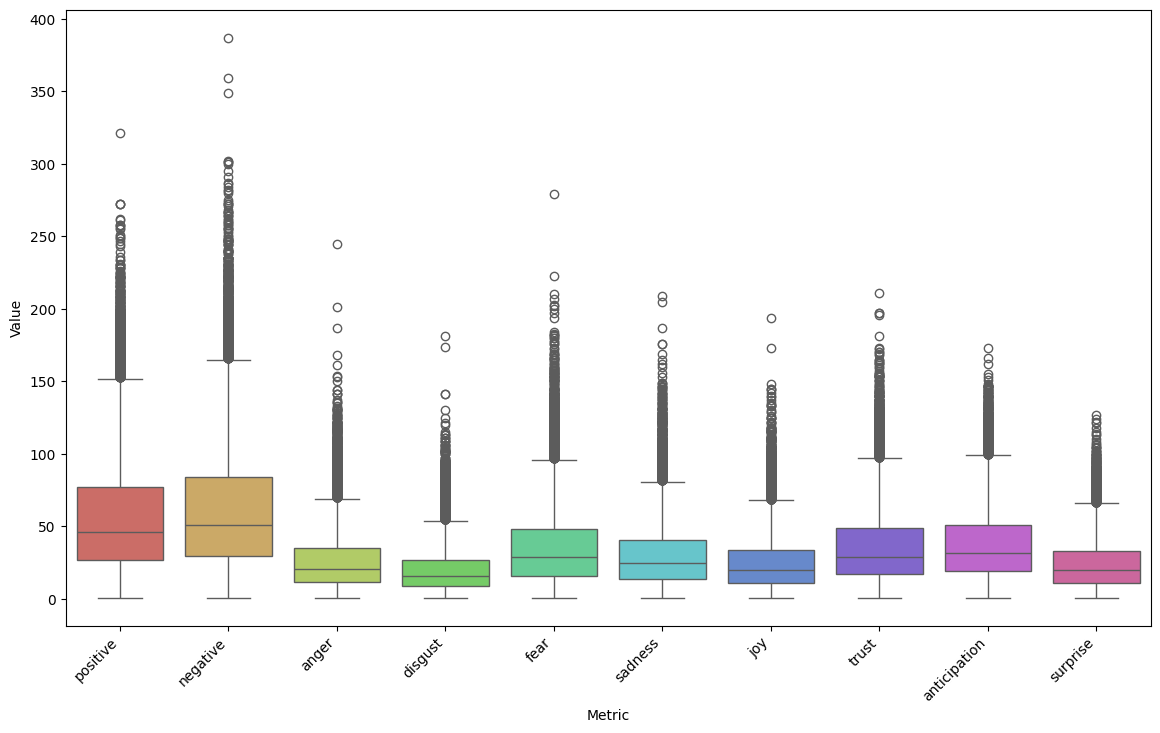
\includegraphics[width=\textwidth]{illustration/emotions.png}
%	 		\caption{Valeurs de la polarité et des sentiments obtenus grâce au \emph{NRC Lex}}
%	 		\label{fig:emotions}
%	 	\end{subfigure}
%	 	\hfill
%	 	\begin{subfigure}[b]{0.45\textwidth}
%	 		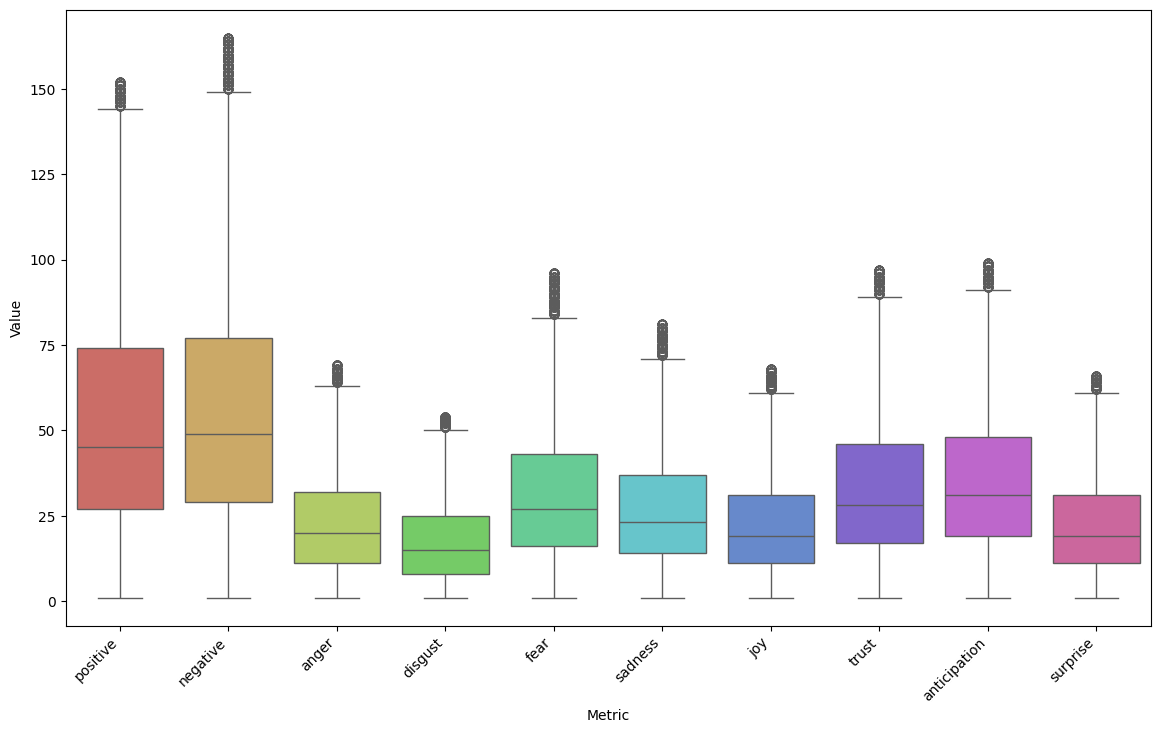
\includegraphics[width=\textwidth]{illustration/emotions_corrected.png}
%	 		\caption{valeurs corrigées de la polarité et des sentiments obtenus grâce au \emph{NRC Lex}}
%	 		\label{fig:emotions_corrected}
%	 	\end{subfigure}
%	 	\caption{score d'émotions et de polarité avant et après correction}
%	 	\label{fig:emotions_both}
%	 \end{figure}
%	 
%	 Avant de rentrer dans la description des résultats, il convient de noter un élément important : la présence abondante de valeur aberrantes. Si elles ne sont pas problématique en soi, elles témoignent de l'existence de textes au valeur significativement plus élevés \footnote{plus d'1,5 fois l'écart interquartile}. 
%	 Afin de rendre les résultats plus lisibles, nous avons choisi de supprimer une partie de ces valeurs aberrantes (qui ne modifient donc pas la dispersion des donnée) (cf. \ref{fig:emotions_corrected})
%
%\subsection{La polarité}
%On remarque rapidement que, la polarité attendue, c'est à dire la polarité négative, n'est que très légèrement supérieure à la polarité positive :  la dispersion de la polarité est plus importante (il existe des textes qui sont "plus négatif" que le maximum de positif). 
%Une hypothèse possible quant à cette répartition de la polarité presque égale tient au fonctionnement de ces histoires : les éléments négatifs caractéristiques, qui amènent la peur et le doute, n'apparaissent que relativement tard narrativement parlant. A l'instar des nouvelles fantastiques, comme nous l'avons précédemment mentionné, le caractère horrifique des CP tient à une situation 'normale"  qui se voit perturbée. Comme nous l'avons noté aussi, la perturbation n'est pas des plus brutale, du moins en ce qui concerne le vocabulaire (cf \ref{section_topic}). Ces éléments peuvent expliquer la question de la polarité.
%	
%
%\subsection{Les sentiments}
%Pour ce qui est des sentiments les résultats sont peut être plus attendus. On retrouve deux émotions fortes : la peur naturellement, et l'anticipation.  Pour ce qui est l'anticipation on peut attribuer cette valeur à nouveau au fonctionnement des CP : une fois la perturbation ou l'élément déclencheur atteint, le doute et donc l'attente d'une résolution va venir prendre la place de la joie par exemple.
%La relative faiblesse des scores du dégout de la surprise ou de la colère nous permet d'étayer l'hypothèse selon laquelle les CP se construiraient presque en opposition aux stéréotypes de l'horreur : la surprise et le dégout, associés à un tueur fou assoiffé de sang laisse sa place à l'attente et l'incompréhension.


\section{Conclusion}
Ce panorama d'outil et de métriques obtenues par méthodes computationelles nous permet de mieux saisir certains éléments de caractérisation des CP. 
\par
D'un point de vue syntaxique et formel tout d'abord,  les CP brillent par leur simplicité : les productions sont très courtes, et accessible. Les phrases courtes et le vocabulaire simple rendent les texte lisibles par le plus grand nombre, ce qui est en accord avec un des éléments de définitions des CP : le rapport à la viralité. Celle-ci semble prendre le pas sur la littérarité d'un point de vue syntaxique : il vaut mieux faire simple, que complexe.

\par Concernant les thèmes, nous avons pu observer une différence majeure avec les stéréotype du genre : les thèmes mobilisés sont ceux de l'expérience, de l'intime et des relations, floutant la limite entre le cadre et l'élément déclencheur de l'horreur.

\par Enfin ces différentes observations nous permettent d'avancer l'idée d'une certaine subtilité dans les productions : le but n'est pas tant de faire sursauter, d'en appeler au gore, mais bien de questionner, de déstabiliser, en mettant en scène le quotidien et l'expérience personnelle, facilitant ainsi l'immersion du lecteur dans le texte.


\chapter[Expliquer le succès]{Expliquer le succès : une tentative de regression logistique}

Toutes les histoires ne se valent pas : au-delà des considérations esthétiques, certaines histoires ont connu une trajectoire plus importante que d'autres. Ce sont les CP historiques que nous avons mentionnés précédemment.

Le but de cette partie est d'explorer les différences entre les deux corpus et de rechercher quels éléments quantitatifs pourraient expliquer le succès d'une histoire par rapport à une autre. Pour ce faire, nous avons procédé en deux temps:
\begin{itemize}
\item  Dans un premier temps, nous avons cherché à identifier parmi les variables calculées précédemment les plus pertinentes pour comprendre les différences entre les histoires. 

\item  Une fois les variables identifiées, nous avons procédé à une analyse statistique pour déterminer l'impact de ces variables sur le succès des histoires. Nous avons utilisé des techniques de régression pour modéliser les relations entre les variables indépendantes (les facteurs identifiés) et la variable dépendante (le succès de l'histoire). 
\end{itemize}

\section{Identification des variables pertinentes}
Afin de réaliser une régression de bonne qualité, il convient de sélectionner des variables à la fois pertinentes et dé-corrélées : en effet, la corrélation des variables peut entraîner des problèmes de multicolinéarité, rendant les coefficients de la régression instables et difficiles à interpréter. Pour ce faire il est nécessaire de réduire le nombre de variable pour ne garder qu'un nombre plus restreint mais plus explicatif. 
Dans un premier temps nous avons agrégé les indices de lisibilités : après avoir normalisé les valeurs, nous en avons fait la moyenne géométrique afin de produire une nouvelle variables. Avant cela nous avons vérifié la corrélation de ces variables afin de vérifier la pertinence d'une telle agrégation : 
\begin{figure}[htbp]
	\centering
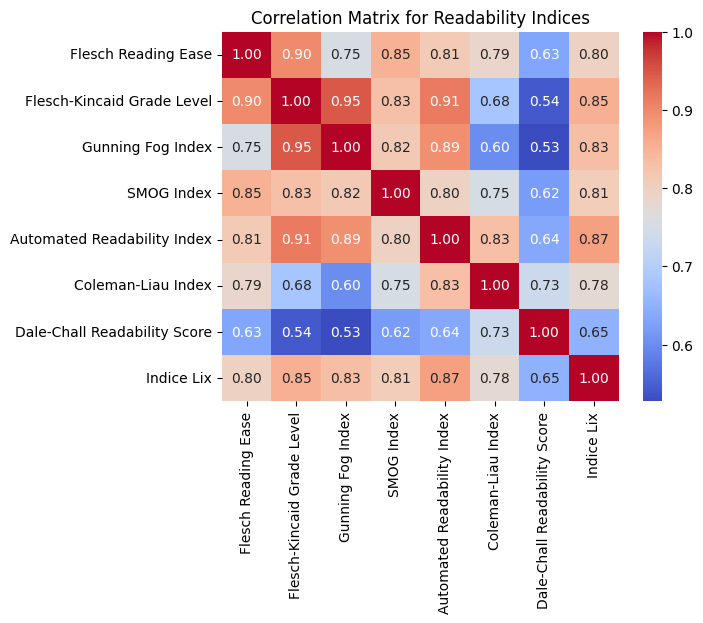
\includegraphics[width=\textwidth]{illustration/corr_read.png}
\caption{Matrice de corrélation des indices de lisibilités}
\label{fig_corrread}
\end{figure}

On remarque que l'indice de Dale-Chall mis à part, les autres indices ont un score très élevé de corrélation : Les indices apparaissent donc comme produisant un résultat similaire. 
Malgré cela,cette agrégation reste artificielle et problématique : une façon plus \og propre\fg{} de procéder consisterait à d'abord vérifier, en plus de la corrélation, la cohérence des indices afin de s'assurer, qu'au delà de la corrélation générale, les indices, au cas par cas, produisent des mesures similaires. Cette nouvelle variable dans notre cas peut être considéré comme un \og proxy \fg{} rapide, dans l'objectif de produire une première analyse statistique.

Une fois cette fusion opérée, la prochaine étape est de vérifier quelles variables sont les plus pertinentes  : cette fois ci la question se pose au-delà des indices mesurant la même chose. Afin de sélectionner les variables les plus pertinentes, nous avons procédé à une première régression dite séquentielle (\emph{stepwise regression}).  Le principe de cette régression est le suivant : l'algorithme part d'une modèle vide et vient ajouter progressivement les variables, tout en mesurant l'effet de la nouvelle variable. Si celle-ci est statistiquement significative elle est conservée. Puis l'inverse est réalisé pour s'assurer de la pertinence des variables sélectionnées : les variables sont enlevées au fur et à mesure tout en suivant la même logique . 

Cette méthode nous permet de réduire le nombre de variables au nombre de  14 : la lisibilité, la longueur des phrases, la tristesse, la peur, la colère, la joie, la joie, la surprise, l'attente, le positif et les topics 2, 3, 4, 9 , 12 (respectivement  : la douleur physique, les animaux de compagnie, la voiture, la forêt et les expériences traumatiques). 

Une fois ces variables sélectionnées, on applique un algorithme de régression logistique sur notre corpus limités aux-dites variables.

\section{Résultats de la régression}
\begin{table}[htbp]
	\centering
	\caption{Résultats de la régression logistique}
	\begin{tabular}{lcccc}
		\toprule
		& \textbf{Coefficient} & \textbf{Std. Err.} & \textbf{z} & \textbf{P>|z|} \\
		\midrule
		const                        & -5.8195 & 0.213 & -27.356 & 0.000 \\
		readability & 5.7874  & 0.463 & 12.503  & 0.000 \\
		longueur\_phrase             & -2.5806 & 0.404 & -6.380  & 0.000 \\
		topic\_douleur\_physique                     & -0.6548 & 0.322 & -2.032  & 0.042 \\
		sadness                      & 0.5662  & 0.149 & 3.802   & 0.000 \\
		fear                         & -0.7814 & 0.184 & -4.252  & 0.000 \\
		anger                        & 0.2779  & 0.147 & 1.888   & 0.059 \\
		topic\_forêt                     & 1.0509  & 0.455 & 2.312   & 0.021 \\
		topic\_voiture                   & -0.7302 & 0.462 & -1.579  & 0.114 \\
		topic\_trauma                 & -1.2659 & 1.005 & -1.260  & 0.208 \\
		positive                     & -0.4414 & 0.185 & -2.389  & 0.017 \\
		joy                          & 0.2468  & 0.145 & 1.700   & 0.089 \\
		anticipation                 & -0.2893 & 0.166 & -1.745  & 0.081 \\
		surprise                     & 0.1851  & 0.129 & 1.436   & 0.151 \\
		topic\_animaux                     & -0.3851 & 0.285 & -1.349  & 0.177 \\
		\midrule
		\textbf{Log-Likelihood}      & \multicolumn{4}{c}{-1724.7} \\
		\textbf{Pseudo R-squared}    & \multicolumn{4}{c}{0.06516} \\
		\textbf{LLR p-value}         & \multicolumn{4}{c}{2.744e-43} \\
		\bottomrule
	\end{tabular}
	\label{table:logit}
\end{table}

\subsection{Les scores globaux}
Afin de mesurer la qualité de la régression, il convient, avant de regarder les variables respectivement, d'analyser les scores globaux de celle-ci. 
Ces 3 scores (\texttt{Log-Likelihood, Pseudo R-squared, LLR p-value}) mesurent respectivement la qualité de l'ajustement aux observées, la proportion de la variance des données explicatives, et si le modèle est significatif par rapport au modèle nul. 
Si le premier score est dure à analyser ( la valeur, sans comparaison ne nous apportent rien), les deux suivants, le \texttt{pseudo R-squared} et la \texttt{LLR p-value} sont elles significatives en soi : la valeur du \texttt{pseudo R-squared} signifie que le modèle explique environ 6.5\% de la variation des données. Cette valeur est faible, sans pour autant qu'elle invalide les résultats. 
En revanche, la valeur du LLR p-value nous indique que le modèle est significatif : le seuil admis pour considérer qu'un modèle est significatif est généralement de 0.05. Ici la valeur de 2,744e-43\footnote{0.00000000000000000000000000000000000000002744} est bien inférieur à ce seuil : les variables explicatives apportent une amélioration substantielle à l'ajustement du modèle par rapport à un modèle nul.

Ces deux conclusions ensemble suggèrent que, bien que le modèle actuel puisse être amélioré en incluant d'autres variables explicatives ou en modifiant la structure du modèle, les variables incluses actuellement sont importantes et apportent une contribution significative à la compréhension du phénomène étudié.

\subsection{Les variables explicatives}
Afin d'analyser les variable explicatives, nous prendrons en compte les valeurs des coefficients et les p-values (\texttt{P>|z|}). Ces deux éléments nous indiquent respectivement le poids de la variable (si le coefficient est positif, la probabilité pour que le texte soit viral augmente, et inversement pour une valeur négative), et si la variable est statistiquement significative (à nouveau le seuil à partir duquel on considérera la variable significative est 0.05 : au-dessus la variable n'est pas considéré comme statistiquement significative).  Ainsi les variables qui vont nous intéresser sont naturellement les variables avec un haut coefficient et une p-value très faible. 
Et deux variables semblent remplir ces conditions : la longueur moyenne des phrases et la lisibilité. D'après le modèle, les histoires virales sont caractérisées d'abord par deux phrases plus courtes (coefficient négatif), mais des indices de lisibilités plus élevés (c'est à dire des textes plus difficile à lire). 
Si ces deux résultats peuvent apparaître comme contradictoire, l'explication possible n'est pas insensée. Une lisibilité accrue signifie une augmentation des mots longs et complexe. Ainsi les histoires virales tendent à concentrer les éléments syntaxiques. Une hypothèse que l'on pourrait émettre teindrait à un travail plus poussé du style de la part des auteurs, où cherchant à produire des phrases simples (dans un soucis d'expression ou de simplicité), on assiste à une sorte  de concentration de la complexité. 

Cette hypothèse va de paire avec l'hypothèse de la subtilité des thèmes et des émotions : la concentration du style irait de paire avec cette subtilité, où plus serait dit avec moins.

Les autres variables, malgré leur faible coefficients restent intéressantes à explorer : Dans un premier temps il convient de noter la quasi absence des thèmes dans les variables explicatives pertinentes. Les thèmes n'apparaissent pas comme un élément vraiment caractéristique. Cette idée est confirmée à la fois par les valeurs des coefficients et par les valeurs relativement élevées des p-value.

Concernant les émotions, le constat est plus nuancé. Surprise mise à part, les émotions semblent être relativement significative. On peut noter l'absence de la valence négative parmi les variables, tout comme une légère pénalité pour la peur et l'anticipation. Ces éléments étaye notre hypothèse : le vocable de la peur ou bien plus négatif n'explique pas le succès, renforçant donc l'idée d'une peur plus subtile.

\subsection{Évolution des variables explicatives les plus significatives}
Enfin en guise de conclusion des computations, nous avons voulu vérifier une dernière hypothèse, concernant le statut canonique de ces histoires : peut-on repérer dans l'évolution de ces métriques un comportement particulier ?
Ces histoires, comme nous l'avons vu précédemment, ont agi comme référence pour les autres histoires. Dès lors, peut-on retrouver cette référentialité dans les métriques que nous avons sélectionnées ? Autrement dit, est-il possible de voir une convergence des métriques dans le temps vers les valeurs des productions historiques ? 
Pour ce faire nous avons calculé le carré de la distance entre la moyenne de l'indice de lisibilité et de longueur de phrase des histoires virales et la valeur de chaque histoire. 
Pour les deux métriques, le schéma est relativement proche : on assiste à une convergence vers la valeur moyenne des histoires virales pour ensuite diverger. 

 \begin{figure}[htbp]
	\centering
	\begin{subfigure}[b]{0.45\textwidth}
		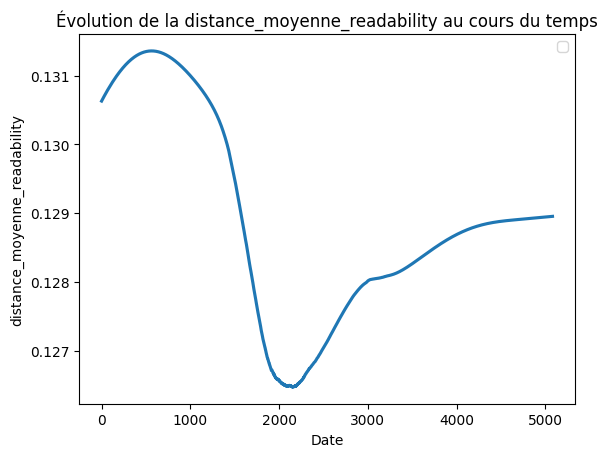
\includegraphics[width=\textwidth]{illustration/distance_lisibilite.png}
		\caption{Évolution de la distance entre la lisibilité et la valeur moyenne des histoires virales}
		\label{fig:distance_lisibilité}
	\end{subfigure}
	\hfill
	\begin{subfigure}[b]{0.45\textwidth}
		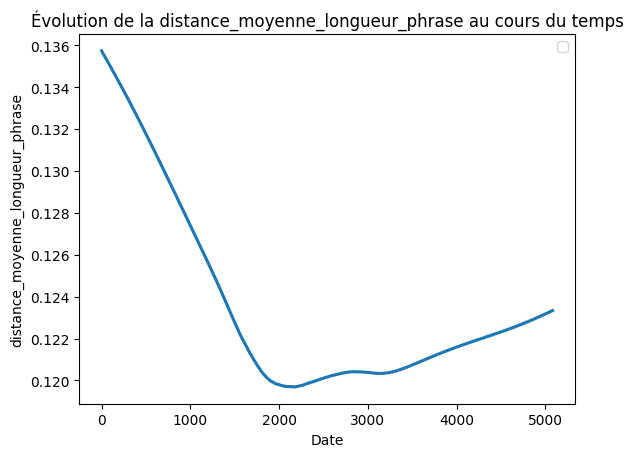
\includegraphics[width=\textwidth]{illustration/distance_phrases.png}
		\caption{évolution de la distance entre la longueur des phrases et la valeur moyenne des histoires virales}
		\label{fig:distance_phrases}
	\end{subfigure}
\end{figure}

Ainsi au cours du temps les histoires vont s'approcher de la forme (une valeur plus basse indique une plus grande proximité) des histoires virales avant de s'en détacher. Si ce ne sont pas des distances entre textes à proprement parler, ces distances permettent d'illustrer, au moins en partie ce phénomène. 

Cette convergence dans notre cas peut être associée à la notion de fécondité qui caractérise les mèmes: les CP virales agissent comme des références et produisent d'autres mèmes. 

Ce schéma n'est pas sans rappeler le schéma obtenu par Cafiero \& Gabay\footcite{cafiero_rise_nodate} dans leur études du théâtre classique : on assiste ici aussi à une convergence vers les références du genre puis à une divergence, ou le genre vient se renouveler et produire une nouvelle façon de faire.

\part{Conclusions, et perspectives futures}
%conclusion
Nous avons amorcé la caractérisation des creepypastas par leur proximité avec la notion de mème, et ces analyses confirment ce rapprochement. Nos analyses ont montré que malgré une forme littéraire, les productions par leur formes étaient caractérisées par leur accessibilité, qualité proche d'un mème à l'ère d'Internet. 

La qualité virale de ces histoires ancrent définitivement celles-ci dans leur aspect numérique, plus que littéraire, sans pour autant renier cet héritage. 
Au contraire : les thèmes et les émotions montrent une plus grande importance de l'intimité. Cette intimité, dans ce genre où narrateur et lecteur semblent ne faire qu'un, rappelle l'intimité plus globale de l'expérience de lecture : même si le lecteur, navigateur sur l'océan du web, passera à autre chose, il apparaît que le temps de cette histoire, il plonge un instant au cœur de cette expérience.

Numériques par la forme, littéraires par l'expérience et virales par construction, les creepypastas sont  un véritable carrefour des genres et des formes.

Ces travaux ne représentent qu'un premier pas, un peu hésitant vers une étude plus approfondie. 
Dans un premier temps, les résultats de la régression nous pousse à continuer notre recherche de variable explicatives de meilleure qualité. 
D'un point de vue purement computationnel, les analyses gagneraient à être plus robuste et à être affiné. Nous évoquions l'agrégation de variables ci-dessus : c'est un exemple d'éléments qui mériterait d'être amélioré.

Le parallèle final avec le théâtre classique n'est pas innocent : un élément que nous avons laissé de côté faute de temps est la présence des règles. Ou plutôt la présence abondante de règles : chaque plateforme a ses règles, mais plus globalement, propose un ensemble de directives à suivre pour produire une creepypasta de bonne qualité. 
La présence de modérateur et de relecteurs qui jugent de la qualité de la production en fonction de ses règles n'est pas anodine. 
L'image anarchique des productions numériques à l'air du web, se voit remplacée momentanément par une organisation massive et stricte. Ces règles sont une porte d'entrée vers tout un pan d'analyse : les règles en soit bien évidemment mais aussi le respect ou non de celles-ci. Quantifier le respect de certaines règles nous permettra d'affiner notre analyses d'histoires virales : émergent-elles des règles ou au contraire, sont-elles à l'origine de celle-ci ? 

	\pagebreak


\backmatter
	\part{Annexe}
	\section*{Données et codes}
	Toutes les données (liens, textes et différents corpus) et tous les scripts et notebooks utilisés sont disponibles à l'adresse \texttt{github} suivante: 
	
	\begin{centering}
		\url{https://github.com/Rollybre/HN_memoire_creepypasta}
	\end{centering}
	\bigskip\\
	\bigskip
	\bigskip
	\section*{Les indices de lisibilité}
\begin{itemize}
		
	\item Flesch Reading Ease : Évalue la facilité de lecture en se basant sur le nombre de mots par phrase et de syllabes par mot. Un score élevé (de 0 à 100) indique une lecture plus facile, tandis qu'un score bas indique un texte plus difficile.
	
	\item Flesch-Kincaid Grade Level : Exprime le niveau de lecture en termes de grade scolaire aux États-Unis. Plus le score est bas, plus le texte est facile à lire.
	
	\item Gunning Fog Index : Mesure la difficulté d'un texte en fonction du nombre de mots par phrase et du pourcentage de mots polysyllabiques. Il fournit un niveau de lecture approximatif.
	
	\item SMOG Index : Évalue la complexité d'un texte en comptant le nombre de mots polysyllabiques dans un échantillon de texte. Le score indique le niveau de lecture estimé.
	
	\item Automated Readability Index : Calculé en fonction du nombre moyen de lettres par mot et du nombre moyen de mots par phrase. Plus le score est bas, plus le texte est facile à lire.
	
	\item Coleman-Liau Index : Détermine la facilité de lecture en évaluant le nombre de lettres par mot et le nombre de phrases par 100 mots. Il fournit un niveau de lecture estimé.
	
	\item Dale-Chall Readability Score : Évalue la lisibilité en fonction du nombre de mots difficiles à comprendre dans un texte. Il est adapté pour les textes destinés à des lecteurs peu expérimentés.
	
	\item Indice Lix : Mesure la complexité d'un texte en évaluant le nombre de mots longs par phrase et le pourcentage de mots courts. Plus le score est élevé, plus le texte est difficile à lire.


\end{itemize}	


	

		\pagebreak
	\begin{table}[htbp]
		\centering
		\caption{Équivalents Scolaires (France) et Indices de Lisibilité en Anglais - Partie 1}
		\resizebox{\textwidth}{!}{%
			\begin{tabular}{cccc}
				\toprule
				\textbf{Équivalence Scolaire} & \textbf{Flesch Reading Ease} & \textbf{Flesch-Kincaid Grade Level} & \textbf{Gunning Fog Index} \\ \midrule
				CP - CE1                               & 90-100                           & 1.0-2.0                               & 6.0-7.0                           \\ 
				CE2 - CM1                              & 80-89                            & 3.0-4.0                               & 7.0-8.0                           \\ 
				CM2 - 6ème                              & 70-79                            & 5.0-6.0                               & 8.0-9.0                           \\
				5ème - 4ème                             & 60-69                            & 7.0-8.0                               & 9.0-10.0                         \\
				3ème - 2nde                             & 50-59                            & 9.0-10.0                              & 10.0-11.0                        \\ 
				1ère - Terminale                        & 30-49                            & 11.0-12.0                             & 11.0-12.0                        \\ 
				\bottomrule
			\end{tabular}%
		}
		\label{tab:readability_indices_part1}
	\end{table}
	
	\begin{table}[htbp]
		\centering
		\caption{Équivalents Scolaires (France) et Indices de Lisibilité en Anglais - Partie 2}
		\resizebox{\textwidth}{!}{%
			\begin{tabular}{cccc}
				\toprule
				\textbf{Équivalence Scolaire} & \textbf{SMOG Index} & \textbf{Automated Readability Index} & \textbf{Coleman-Liau Index} \\ 
				\midrule
				CP - CE1                               & 4.0                               & 1.0-2.0                                     & 1.3-2.8                                 \\ 
				CE2 - CM1                              & 5.0                               & 3.0-4.0                                     & 3.0-4.5                                 \\ 
				CM2 - 6ème                              & 6.0                               & 5.0-6.0                                     & 5.0-6.5                                 \\ 
				5ème - 4ème                             & 7.0                               & 7.0-8.0                                     & 7.0-8.5                                 \\ 
				3ème - 2nde                             & 8.0                               & 9.0-10.0                                    & 9.0-10.5                               \\ 
				1ère - Terminale                        & 9.0                               & 11.0-12.0                                   & 11.0-12.5                             \\ \bottomrule
			\end{tabular}%
		}
		\label{tab:readability_indices_part2}
	\end{table}
	
		
	
	



	\section*{Les indices de richesse lexicale}
	\label{annexe_richesse_lex}
	\begin{itemize}
		
	\item Ratio Types/Tokens : Évalue la richesse lexicale en comparant le nombre total de mots distincts au nombre total de mots. Un ratio élevé indique une plus grande variété de mots utilisés.

\item Hapax Legomena : Nombre de mots n'apparaissant qu'une seule fois dans un texte, indiquant la variété du vocabulaire et la rareté des mots utilisés.

 \item Densité Lexicale : Mesure la proportion de mots uniques dans un texte par rapport au nombre total de mots. Une densité plus élevée indique une plus grande variété lexicale.

 \item Indice Honore's R : Calculé en divisant le nombre de mots uniques par la racine carrée du nombre total de mots, pour évaluer la richesse lexicale ajustée à la longueur du texte.
	\end{itemize}

			\pagebreak
			\nocite{*}
	\printbibliography
\end{document}
